\chap{Evaluating the Efficacy with Patient Population} \label{chapter: prevention-rctresults}

\setlength{\epigraphwidth}{.50\textwidth}
\begin{epigraphs}
\qitem{It remains an ideal that all new healthcare interventions should be evaluated through randomised controlled trials.}
{--- \textsc{Prof. Bonnie Sibbald} \\ \textit{Former Chair of the UK Health Services Research Network}}
\end{epigraphs}

This chapter details the results from a 6-month randomised control trial (RCT) which aimed to reduce participant's AD risk in later life, using the developed Gray Matters app.

\section{Introduction}
To truly evaluate the mobile behaviour change intervention framework, it must be used within it's intended environment, with it's intended user population. With the framework applied to the application area of AD, the Gray Matters app was created, and subsequently evaluated from a technology viewpoint, by expert raters in the domain area. The final test of efficacy is within the apps use as a tool to change behaviour with an appropriate study cohort. As such an RCT was designed to evaluate the app over 6-months with a cohort of 144 persons\footnote{ClinicalTrials.gov Identifier: NCT02290912}.

\section{Study Design}
The study was an RCT; delivered over a 6-month period, commencing in April 2014, with post-test collection performed at the close.
The study was designed as an intervention, and consisted of subjects who were randomly assigned into either treatment or control groups. Those assigned to the treatment group were given access to the Gray Matters app, and additional intervention components. The treatment group were not given a strict regimen and therefore a wide range of engagement levels were anticipated. The control group were not given access to any intervention components and were used for baseline comparisons. A uniform random number generator (0,1) within SPSS v21 was used to randomize participants into treatment and control groups, with the aim of allocating 1/3 of the participants to control, and 2/3 to treatment.

\subsection{Recruitment}
Recruitment of participants was achieved by emailing announcements to faculty, alumni and staff of Utah State University and distributing flyers at health fairs and other venues, assisted by the local health department and their community liaisons. For those interested a pre-screening eligibility survey was completed. Eligibility criteria included:
\begin{enumerate}[noitemsep,topsep=0pt,label=(\alph*)]
\item Age between 40 and 64 years.
\item BMI no higher than 41.
\item Possession of a smartphone or tablet (iOS or Android only)
\item Fluency in the English language
\item Residence in Cache County, Utah, United States of America.
\item Not having any of the following medical conditions: pregnancy, dementia, unmanaged diabetes, or untreated major depression.
\end{enumerate}

\subsection{Statistical Power}
To achieve 80\% statistical power to detect a medium effect size (Cohen's d=.50) when comparing the difference between two independent means at a 2:1 (treatment:control) ratio, 96 treatment and 48 control (144 total) participants were needed, calculated using G*Power \cite{Faul2007}. Upon randomisation participants were allocated to each group, however, to avoid intra-couple contamination of intervention material, married couples were assigned to the same randomised group (n=12). This adjustment resulted in 104 participants assigned to treatment and 42 to control, resulting in an approximate 5:2 ratio (treatment:control).

\subsection{Outcome Measures}
Outcome measures for the RCT study were categorised as primary, secondary, and tertiary outcome measures.
\newline Primary outcome measures included a set of anthropometric measures and blood-based biomarkers that are associated with AD onset in the literature. All measures are continuous variables, however, they have been categorised into categorical variables where appropriate, as shown in Table \ref{tbl: clinical-variables}.
\newline Secondary outcome measures included behavioural measures conducted through a battery of tests to assess metacognition, motivation, readiness-for-change, sleep quality, social engagement, depression, and couple satisfaction (among married persons), and are detailed in Table \ref{tbl: behavioural-variables}.
\newline Tertiary outcome measures include app statistics derived from analytical code, including time spent using app, number of launches per week, and usage patterns. Demographic variables were also recorded, examples include gender, ethnicity, marital status and house hold income, and are detailed in Table \ref{tbl: demographic-variables}.
\newline Tables containing full summaries of all recorded values at the beginning of the study, for all 146 Gray Matters study participants, are detailed by \citeauthor{Norton2015-TRCI} in \cite{Norton2015-TRCI}.

\begin{table}[]
\centering
\caption{Clinical and laboratory biomarkers recorded for each participant}
\label{tbl: clinical-variables}
\begin{tabular}{@{}ll@{}}
\toprule
Measures & Categorical (where appropriate) \\ \midrule
Body Mass Index (kg/m\textsuperscript{2}) & \begin{tabular}[c]{@{}l@{}}Underweight, Normal \\ Overweight, Obese (Class I-III)\end{tabular} \\
Systolic blood pressure (mmHg) & N/A \\
Diastolic blood pressure (mmHg) & Low, Ideal, Pre-High, High \\
Pulse (bpm) & N/A \\
C-reactive protein (mg/L) & N/A \\
Glucose, serum (mg/dL) & N/A \\
Insulin ($\mu$IU/mL) & N/A \\
HDL cholesterol (mg/dL) & Low, Medium, High \\
LDL cholesterol (mg/dL) & \begin{tabular}[c]{@{}l@{}}Optimal, Near Optimal \\ Borderline High, High, Very High\end{tabular} \\
Total cholesterol (mg/dL) & N/A \\
Triglycerides (mg/dL) & N/A \\ \bottomrule
\end{tabular}
\end{table}


\begin{table}[h]
\centering
\caption{Behavioural variables recorded for each participant based on self-rated physical, cognitive, social, emotional and nutritional health}
\label{tbl: behavioural-variables}
\begin{tabular}{@{}ll@{}}
\toprule
Measure & Scale \\ \midrule
Overall physical health & 1-3 \\
Metacognition (memory now vs. 3 years ago) & 1-4 \\
Lifestyle Change Priority & \\
\textit{- Physical Activity} & 1-5 \\
\textit{- Healthy Food Choices} & 1-5 \\
\textit{- Stress Management} & 1-5 \\
\textit{- Cognitive Stimulation} & 1-5 \\
\textit{- Sleep Quality} & 1-5 \\
\textit{- Social Engagement} & 1-5 \\
NIH Toolbox SOCIAL &  \\
\textit{- Emotional Support} & 8 - 40 \\
\textit{- Friendship} & 8 - 40 \\
\textit{- Loneliness} & 5 - 25 \\
\textit{- Hostility} & 8 - 40 \\
Pittsburg Sleep Quality Index \cite{Buysse1989} & 0 - 21 \\
Perceived Stress Scale \cite{Cohen1983} & 0 - 56 \\
CES-D Depression scale \cite{Radloff1977} & 0 - 60 \\
Situational Motivational scale \cite{Guay2000} & 1 - 7 \\
R-URICA Readiness for change scale \cite{McConnaughy1983} & 0 - 10 \\
Couple Satisfaction Index \cite{Funk2007} & 0 - 160 \\
Dietary Approaches to Stop Hypertension (DASH) score \cite{Block1990} & 0 - 40 \\ \bottomrule
\end{tabular}
\end{table}

\begin{sidewaystable}
\centering
\caption{Demographic categorical variables recorded for each participant}
\label{tbl: demographic-variables}
\resizebox{\textwidth}{!}{%
\begin{tabular}{@{}ll@{}}
\toprule
Variable                                                 & Categories                                                                                                                 \\ \midrule
Gender                                                   & Male / Female                                                                                                              \\
Race                                                     & White / Black or African American / Asian /  Native Hawaiian or Other Pacific Islander /American Indian / Other            \\
Marital status                                           & Married / Widowed / Divorced / Never Married                                                                               \\
Religious Affiliation                                    & Catholic or Protestant / LDS (Mormon) / Atheistic or Agnostic / Other (Jewish, Eastern, Other)                             \\
Education                                                & High School / College or Trade/ College B.S. or B.A. graduate/ Graduate or professional                                    \\
Income                                                   & \textless \$45k \$45-55k / \$55-75k / \textgreater \$75k                                                                                  \\
Family history of dementia                               & None/ Mother or Father/ Mother and Father/ Maternal GP or Paternal GP / Maternal GP and Paternal GP / Aunt, Uncle, Sibling \\
Dementia caregiving                                      & Never / Yes, but in past / Yes, currently                                                                                  \\
Smart device in treatment group  & iPhone / iPad /android phone / android tablet (Not mutually exclusive)                                                                              \\
Education                                                & High School / College or Trade/ College B.S. or B.A. graduate/ Graduate or professional                                    \\ \bottomrule
\end{tabular}}
\end{sidewaystable}

For the purposes of this chapter, these outcome measures are categorised into 3 overlapping categories, and are discussed later within the chapter:
\begin{enumerate}[noitemsep,topsep=0pt]
	\item App Usage
	\item Behaviour Change
	\item Clinical
\end{enumerate}

\subsection{Intervention Components}
In addition to the aforementioned Gray Matters smartphone app, participants in the treatment group also had access to a number of additional components to encourage engagement with the study. These included a wrist-worn activity monitor, booster-events, a personal coach and a study website.

\subsubsection{Smartphone App}
The Gray Matters app was used within the study, however, the method of distribution to the cohort was modified from that outlined in the framework in Chapter \ref{chapter: intervention-framework}. For the purpose of the clinical study, the decision was made to exercise additional control over the accessibility of the app. The app was not distributed via public app stores, but rather by using a testing-platform named TestFlight\footnote{Since the study, Apple Inc. have purchased the company and it is accessible to Apple Developers only via \url{https://developer.apple.com/testflight/}}. In order for participants to download the application from TestFlight, they first needed to register an account with the service and request access to the app. This access request then had to be approved by the trial co-ordinators. These additional security steps did cause some issues for the participants during their on-boarding with the study. Nevertheless, the app was successfully downloaded and installed by all 104 participants in treatment, with weekly installations displayed in Figure \ref{fig: number-installs}.

\begin{figure}[h]
    \centering
    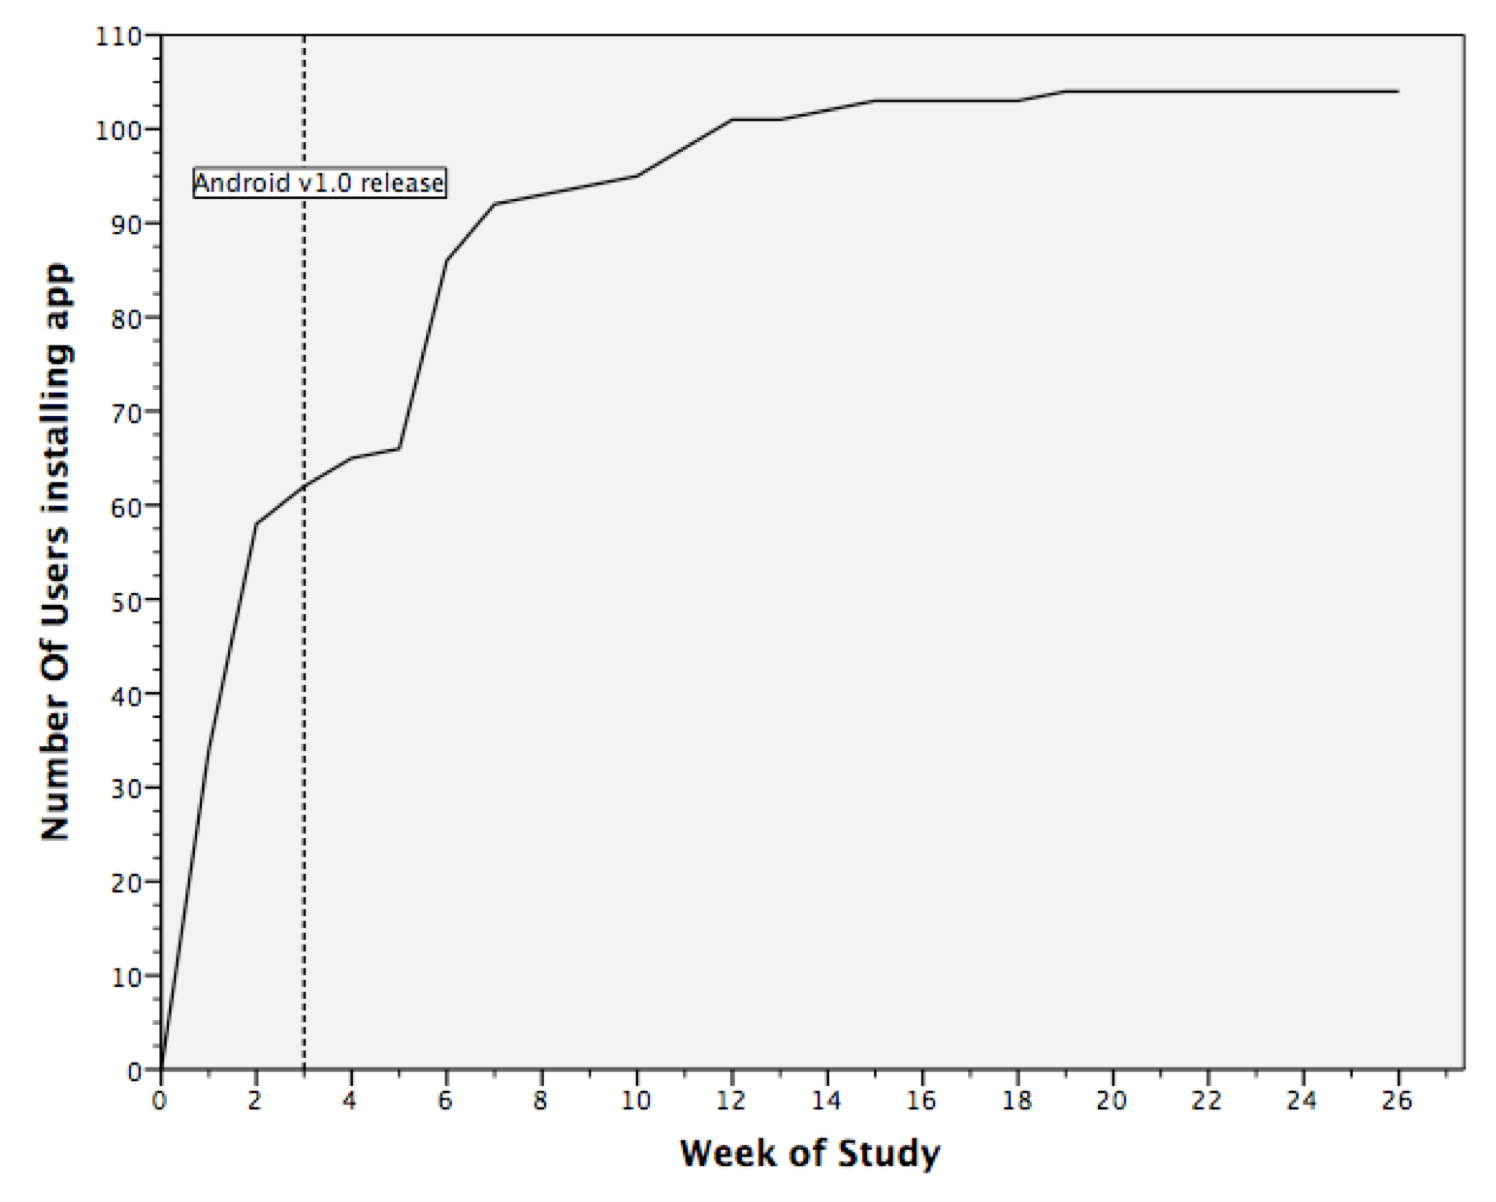
\includegraphics[scale=0.25, angle=0]{Files/prevention-study-3/figures/installs-by-week}
    \caption{Line graph showing number of total installs by week}
    \label{fig: number-installs}
\end{figure}

\subsubsection{Wearable Activity Monitor}
A wearable activity monitor was desired, both as a motivational factor but also as a means to validate self-reported behaviours. The Nike Corporation donated 150 Nike+ FuelBand SE activity monitors, hereafter referred to as FuelBands \footnote{For technical specifications refer to manual available online at \url{https://support-en-us.nikeplus.com/app/answers/detail/a_id/21032/p}}, for the purpose of the study. Each participant was given a FuelBand. This device is worn on the wrist and serves to collect information on physical activity performed throughout the day, such as steps taken, stairs climbed and total minutes of activity. This information is then consolidated into Nike's proprietary metric of ‘Fuel Points’. This device not only serves to collect data, however, also acts as a physical reminder and motivator to increase levels of activity. Participants were asked to manually enter their total number of Fuel Points earned at the end of each day via the smartphone’s log tab.

\subsubsection{Booster Events}
All participants had the option of attending organised booster events. A booster event was designed to emphasize the link between specific actions of a behavioural domain, and the positive effect they had to minimising AD risk. This typically included examples of activities that could be applied in the participants daily routine. For example, a booster event that focused on the food domain hosted cooking classes that promoted sustainable healthy eating choices, whilst educating attendees about the link between the ingredients and AD risk. In total 46 booster events were organised and delivered across the 6-month intervention period. Attendance for each event can be seen in Figure \ref{fig: booster-attendance}.

\begin{figure}[h]
    \centering
    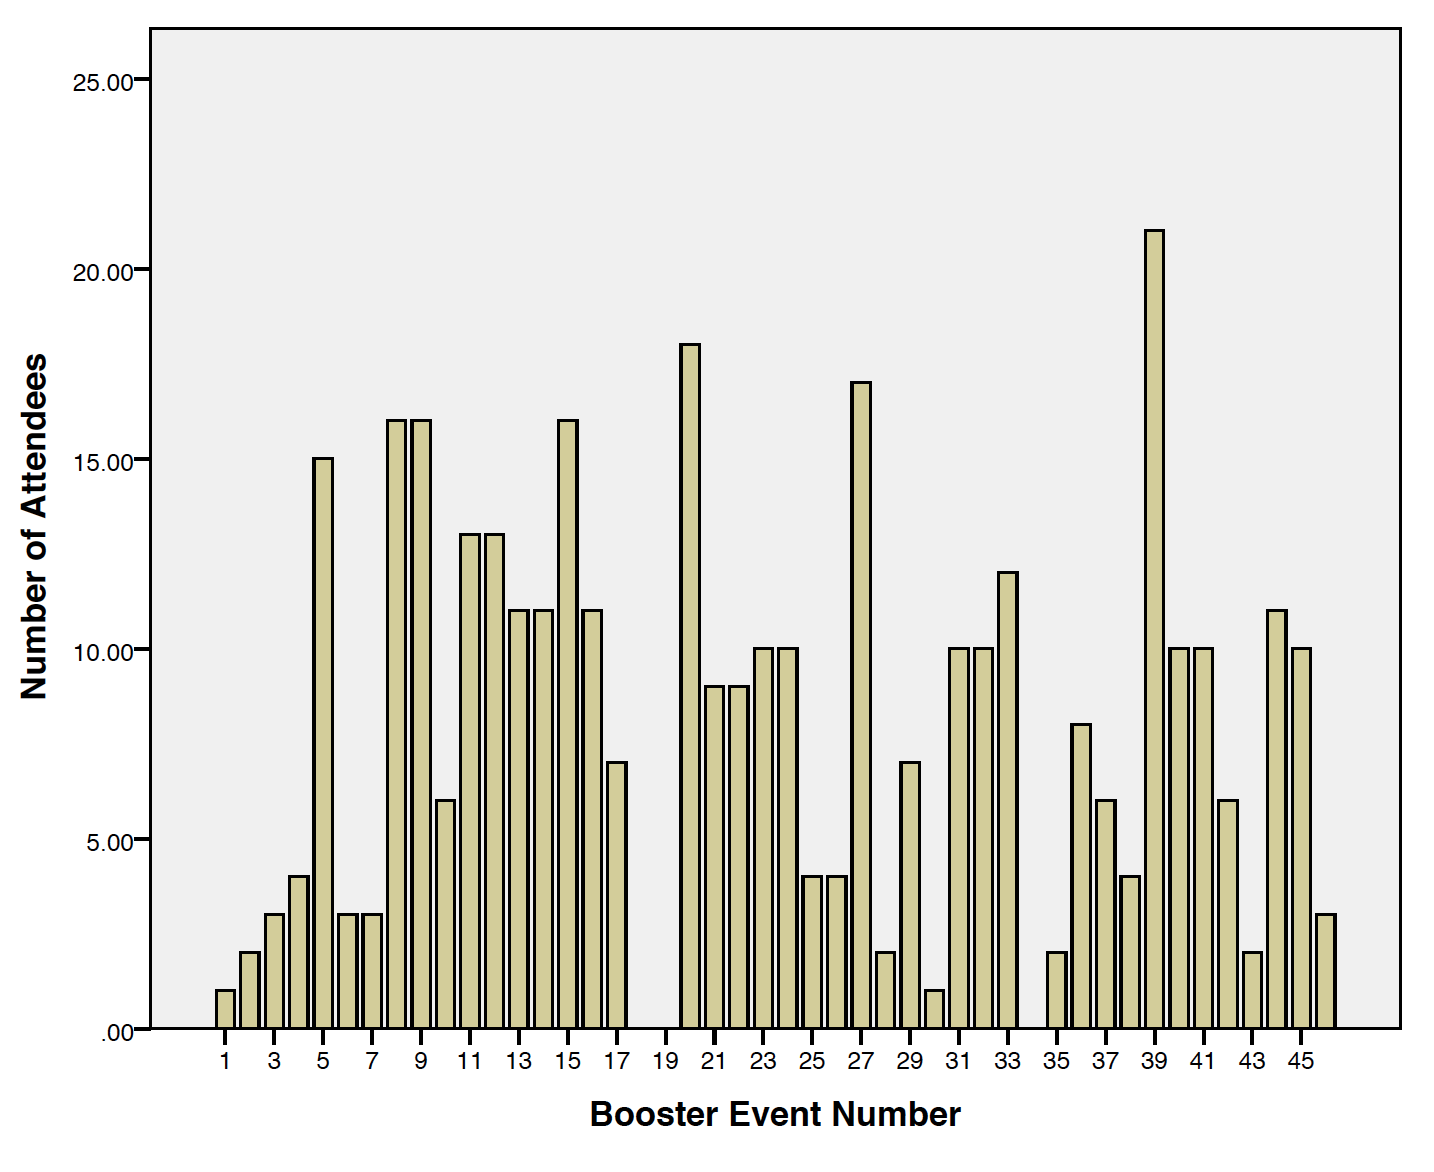
\includegraphics[scale=0.5, angle=0]{Files/prevention-study-3/figures/booster-attendance.png}
    \caption{Bar graph showing attendance numbers of each booster event}
    \label{fig: booster-attendance}
\end{figure}

As seen in Table \ref{tbl: booster-domain-freq}, the majority of booster events where focused on the Physical domain, followed by Food and Stress. The attendance figures however, show the most popular domains with regards to attendance were Sleep and Cognitive.

\begin{table}[h]
\centering
\caption{Frequency statistics of domains targeted and attendance figures at booster events}
\label{tbl: booster-domain-freq}
\begin{tabular}{@{}lllll@{}}
\toprule
Domain & Frequency & Percent & \begin{tabular}[c]{@{}l@{}}Attendance \\ (Mean)\end{tabular} & \begin{tabular}[c]{@{}l@{}}Attendance \\ (Std. Dev)\end{tabular} \\ \midrule
Physical & 15 & 32.6\% & 6 & 5.07 \\
Food & 9 & 19.6\% & 5.78 & 4.81 \\
Social & 2 & 4.3\% & 6.50 & 4.95 \\
Sleep & 4 & 8.7\% & 12 & 3.16 \\
Cognitive & 7 & 15.2\% & 12.14 & 6.14 \\
Stress & 9 & 19.6\% & 8.78 & 5.11 \\ \bottomrule
\end{tabular}
\end{table}

\subsubsection{Personal Coach}
Participants also had access to a personal coach whom they could contact if they required assistance with any aspect of the behavioural domains. A team of 28 student interns with majors in the six behavioural domains volunteered to be personal coaches. Student coaches were trained in motivational interviewing and the transtheoretical model. Where needed, the coaches provided weekly email or text message exchange with their assigned participants to provide emotional support and encouragement for lifestyle change goals. This component of the study was however vastly under-utilised, with many participants reporting at the study close that they did not know they had the facility \cite{Weyerman2015}.
% 11.11.15 - Emailed Maria regarding statistic on how many used the coach. No results yet.

\subsubsection{Study Website}
Participants also had access to a password protected website \cite{Norton2014} that provided supporting material to aid the use of the app and wearable device, which included instructional YouTube videos providing walkthroughs of the Gray Matters app for iOS and Android. In addition an email address was provided should additional issues arise.

\subsubsection{Exit Survey}
An exit survey was designed to capture opinions of participants in the treatment group. The survey asked questions about app usage, motivations, their perceived behaviour change and social network usage. At the end of the study 98\% (n=102) of the participants completed this survey.

\section{App Usage}
A mixture of open-source, and proprietary analytical tracking tools developed by the author were embedded into the runtime code of the apps. This allowed for numerous events, and in-app actions to be tracked over the period of the study. Using this data it was possible to determine levels of adoption, time spent using the app, behaviour patterns when self-reporting, and general patterns of app usage.

\subsection{Adoption}
In Week 1 (10th April 2014) the first iOS version of the app was released to the treatment group. This was performed through a launch event, in which attending participants were instructed how to signup and download the application through the TestFlight platform. By the end of week 1, 31.7\% (n=33) participants had installed the app onto their iPhone and/or iPad. In week 3 (13th May 2014), the first Android version of the app was released to the treatment group due to demand from android users. 2 weeks after this release, 19.2\% (n=20) participants had installed the first version of the Android app. By week 10, 86.5\% of the treatment group (n=90) had installed an iOS or Android version of the app onto their smartphone and/or tablet, with the remainder shortly afterward, as seen in Figure \ref{fig: number-installs}. Many users opted to install the Gray Matters app on both their smartphone and tablet.
Of the 104 users using the app, at the end of the study, 75.97\% of all Gray Matters app sessions were on iOS devices (iPhone: 54.7\%; iPad: 21.27\%) and the remainder on Android devices (24.03\%).

\subsection{Duration of Use}
The average duration of each session with the app, across all devices, is 1 minute 55 seconds. This time is under the originally specified goal of 2 minutes for a user's session duration.

\subsection{Self-Reporting}
Over the duration of the study, over 122,719 behavioural logs were uploaded to the central database. The average user answered 7.3 $ \pm $ 3.16 questions per day during their participation in the study. To further understand the self-reporting process, additional analytical tracking code was added to the app in Week 18. This allowed the investigators to analyse specific behaviours when answering questions in the log screen. One function allowed investigators to quantify the number of times the user altered their behavioural values. Figure \ref{fig: bargraph-questionedits} shows the mean number of times each domain's questions were updated in the self-reporting screen.

 \begin{figure}[h]
    \centering
    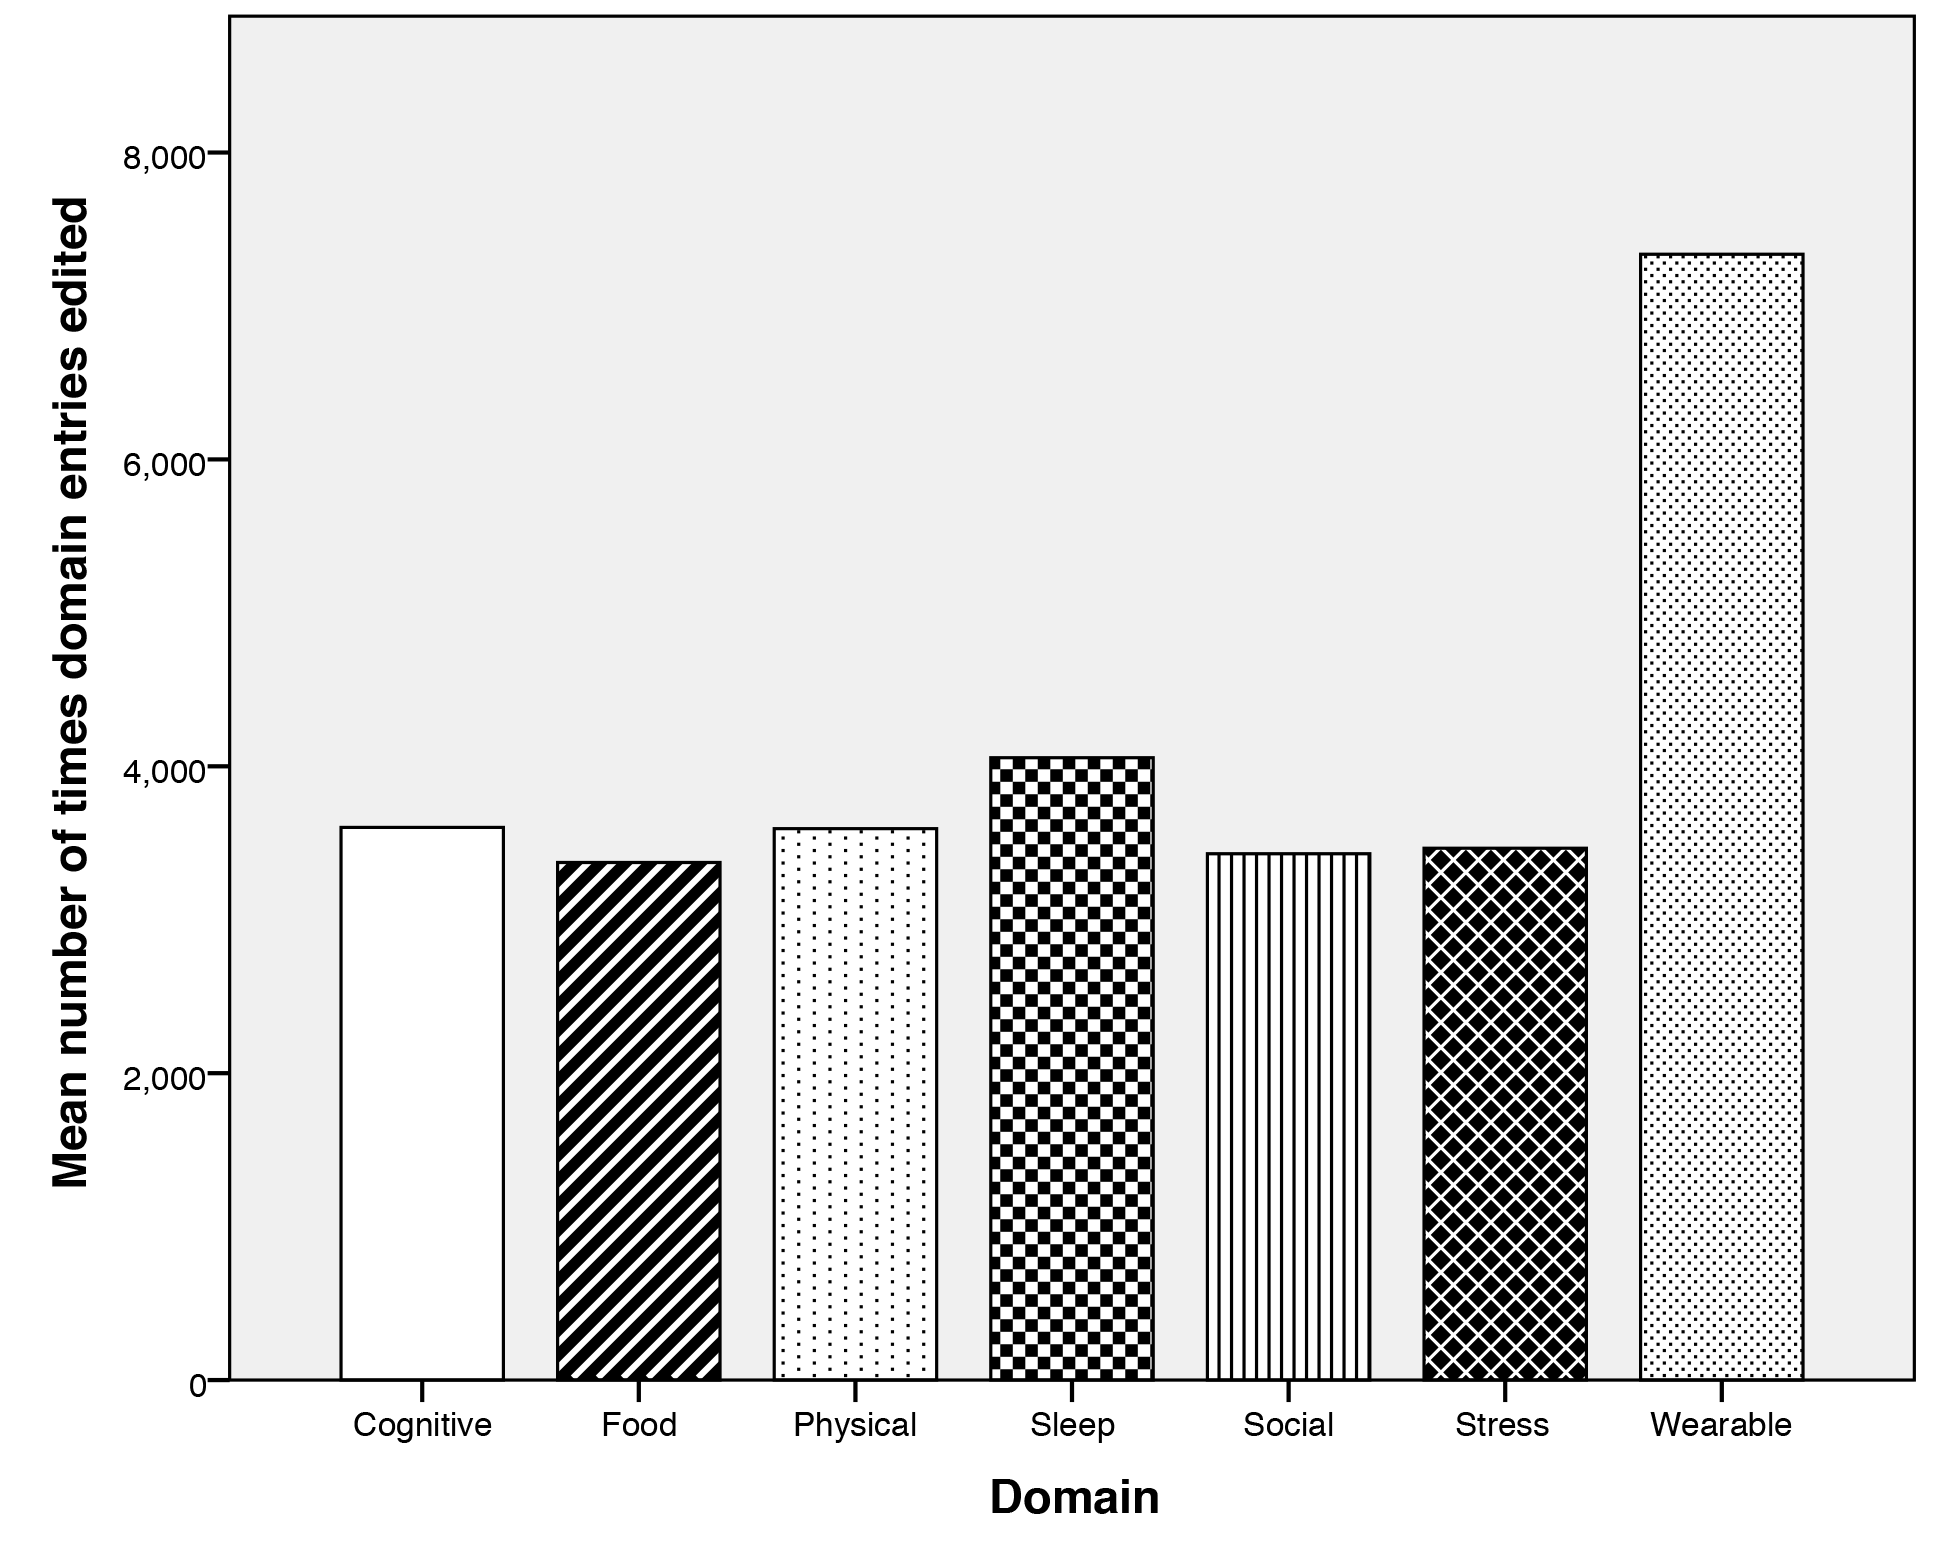
\includegraphics[scale=0.2, angle=0]{Files/prevention-study-3/figures/domain-edits}
    \caption{Bar graph showing the mean number of times each domain’s questions were edited using the sliders in the log screen, using updated analytical code, from week 18 to study end. The wearable domain is updated almost twice as often as the other domains.}
    \label{fig: bargraph-questionedits}
\end{figure}

Across all users in the study, Question 12 was altered a statistically significant amount more than the rest (z = 3.054, p = .0023). Question 12, belongs to the Wearable domain and relates to the number of Nike fuel points earned. It is assumed that users frequently updated this amount, more than the others, due to the variability in the data generated from the wearable device each day when they were active. This also indicates that integration with the wearable devices at a communications level would greatly reduce the need for participant interaction.

\subsection{Time of Day} \label{subsection: time-of-day}
Analytical tracking code also enabled the investigators to observe the patterns of usage with relation to time of day. Figure \ref{fig: time-of-day} shows that usage peaks at 2 points in the day, the first in a short period in the morning around 7-9am. In the evening, however, app usage rapidly increases around 8pm and declines sharply after 11pm. It is believed that the users wait until the end of the day before entering their log data, so that it is the most valid representation of their behaviours in that daily period.

 \begin{figure}[h]
    \centering
    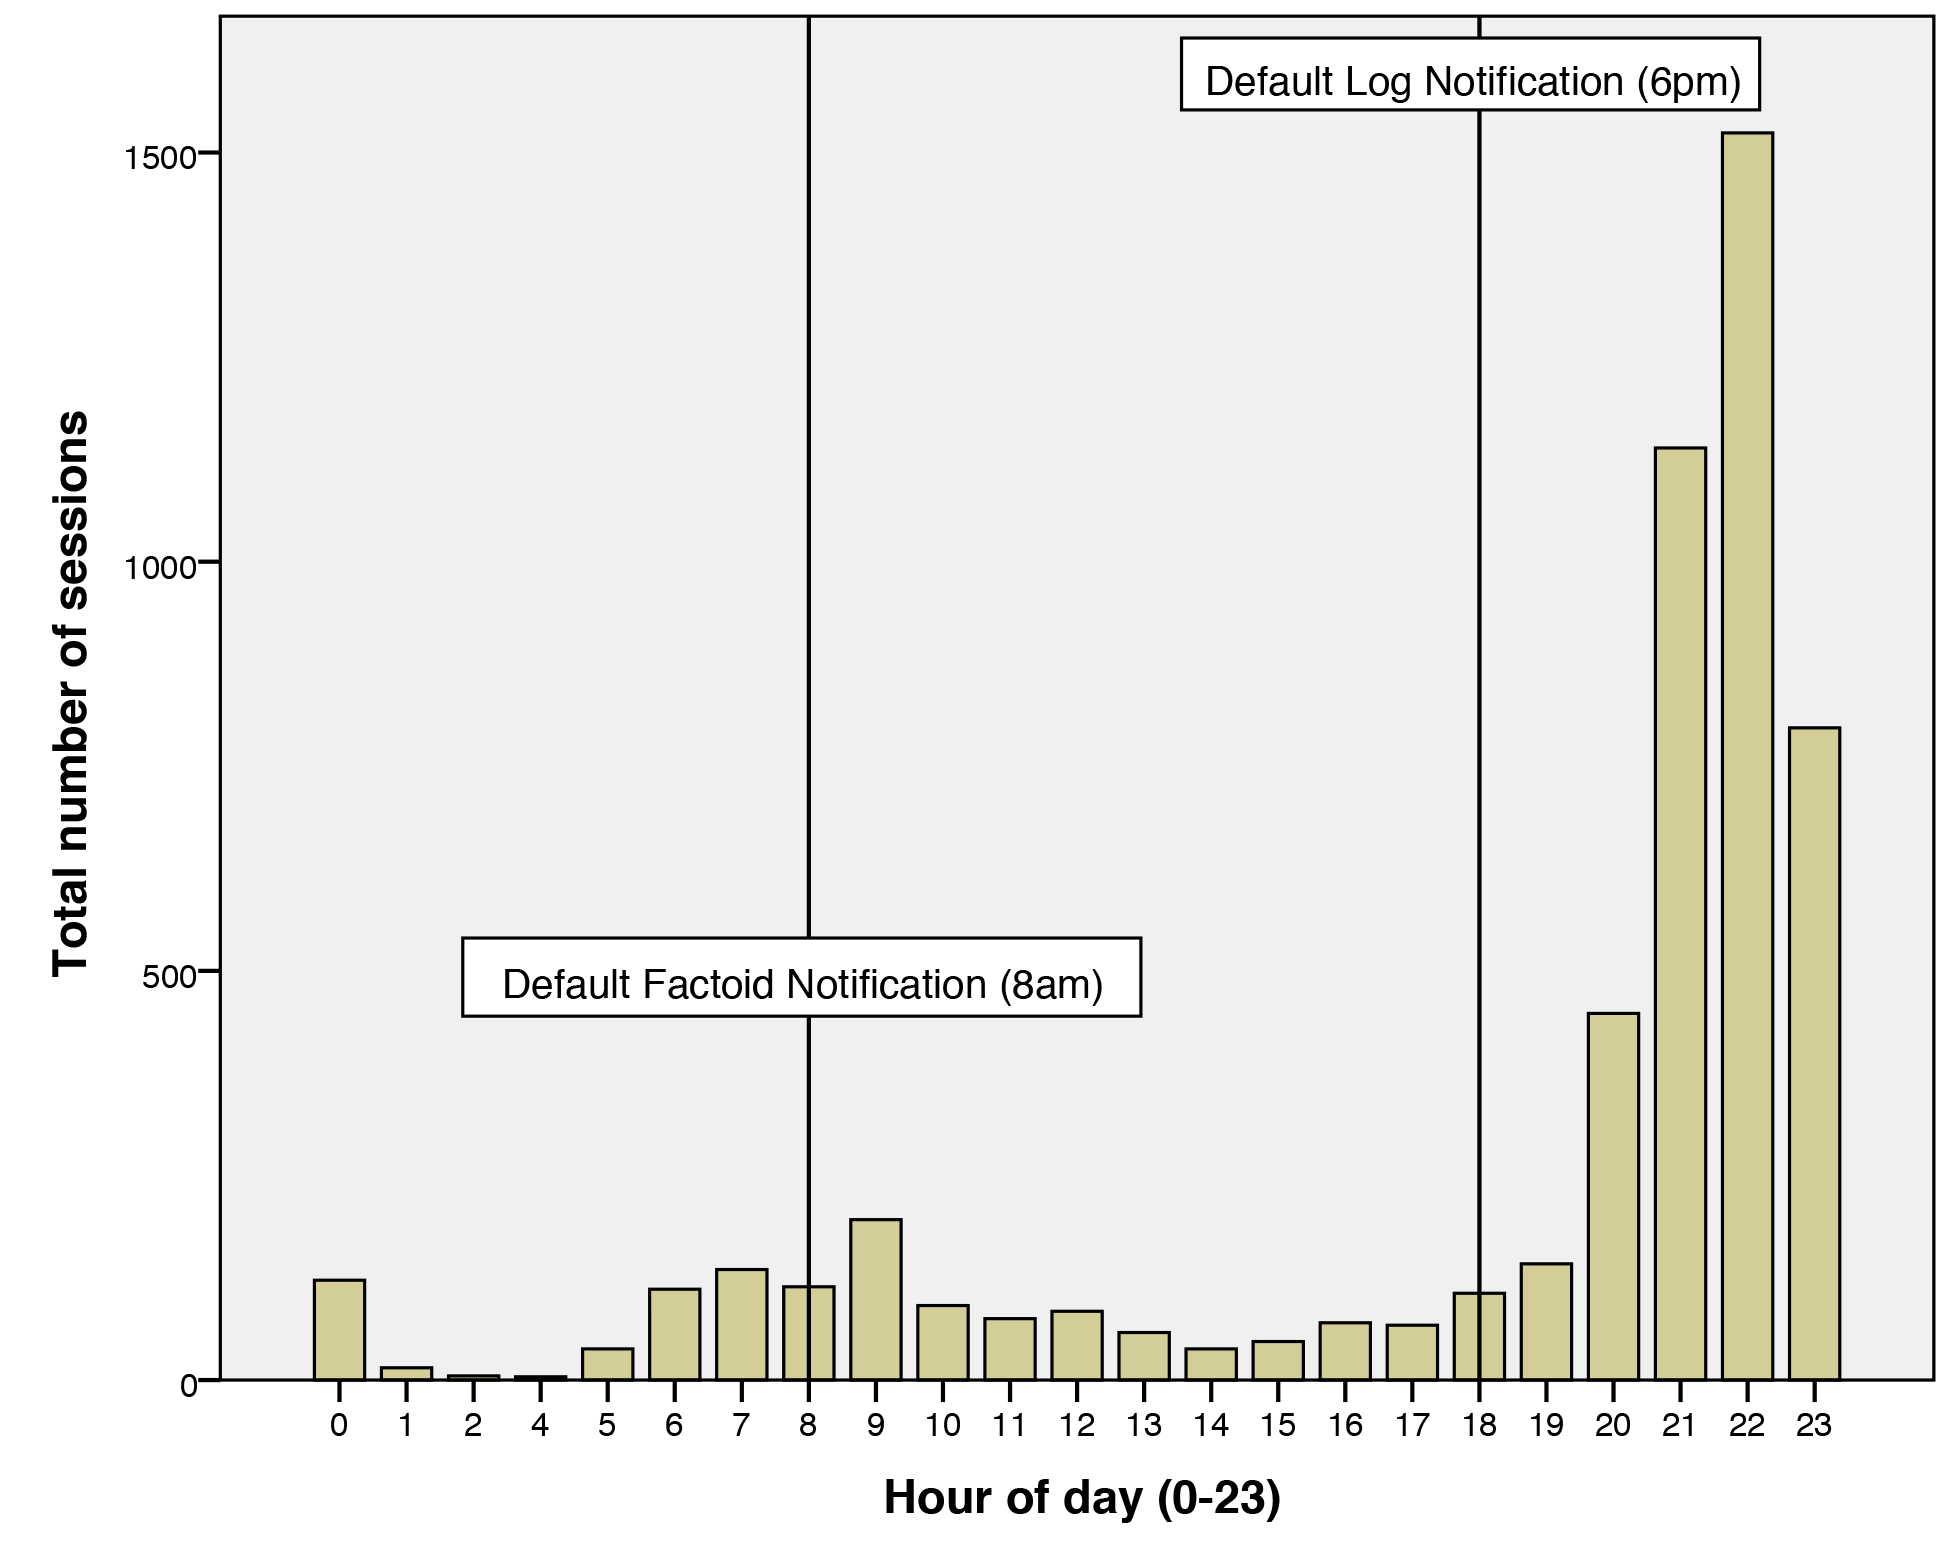
\includegraphics[scale=0.18, angle=0]{Files/prevention-study-3/figures/hour-of-day}
    \caption{Bar graph showing the typical hours of use, with morning activity around the default daily fact notification time at 8am, and activity peaking at 10pm, 4 hours after the default log notification time.}
    \label{fig: time-of-day}
\end{figure}

An additional explanation to these observations may be due to notifications, for which the app was distributed with 2 default times. The first notification was issued in the morning at 8 am, which reminded the user to check their daily daily fact. The second notification was issued at 6pm, which reminded the user to complete the questions in the app’s log tab. These times have been highlighted in Figure \ref{fig: time-of-day}.

\section{Platform Assessment by Users}
Upon the close of the study, an exit survey was issued to those in the treatment group. 41 participants completed the survey. The survey acted to gather users’ motivations for behaviour change and thoughts on the various components of the study, how they used them, and where they felt improvements could be made.

\subsection{Reported Usage}
Firstly, users were asked how often they used the app on a daily, weekly and monthly basis. Results can be seen in \ref{tbl: exit-survey-appusage}. Mean usage figures show that the app was used for approximately 5.5 months, almost twice daily. The largest amount of standard deviation was found in the responses for times per day (3.12).

\begin{table}[h]
\centering
\caption{Respondents' answers to survey question: ``Over the six month Gray Matters intervention period (April 2014 – October 2014), how often did you use the App?"}
\label{tbl: exit-survey-appusage}
\begin{tabular}{@{}llll@{}}
\toprule
              & N  & Mean & Std. Dev. \\ \midrule
Months Used   & 39 & 5.54 & 1.315     \\
Days Per Week & 38 & 6.21 & 1.695     \\
Times Per Day & 38 & 1.66 & 3.122     \\ \bottomrule
\end{tabular}
\end{table}

\subsection{Effect on Motivations}
In addition, the survey acted to glean how the app altered motivations towards various parts of the intervention. The survey revealed that the app motivated users to perform physical activity (Never: 14.6\%, Rarely: 12.2\%, Sometimes: 24.4\%, Often: 31.7\%, All of the time: 17.1\%) and make healthier food choices (Never: 12.5\%, Rarely: 2.5\%, Sometimes: 17.1\%, Often 48.8\% and All of the Time: 17.1\%).

\subsection{Maintaining Effort}
When queried upon the apps effect on their past, current and future behaviours, 46.3\% said they definitely will continue with their physical activity changes, and 31.7\% want to continue and increase their activity; 46.3\% wish to continue their improved eating habits, with 29.3\% wanting to continue and improve.

\subsection{Feature Wishlist}
To improve the overall quality and desirability of the app, users were asked about features that they wish were included in future versions.
68.3\% of users wished that guidelines were based on their ‘current’ health status, 34.1\% wished they could set their own target goals, 53.7\% wished they could focus the daily facts on specific behaviour goals of interest and 51.2\% wished to received text feedback if they had made good progress/no progress. 53.7\% wished they could compare their behaviours with others relative to their age, gender and initial fitness status. Regarding the wearable device and app interaction, 70.7\% of post-study survey respondents wished that their wearable automatically synched to the app.
These requested features further emphasise the need for social and wearable integration, and reflect the observations and recommendations made within the app content-analysis performed in Chapter \ref{chapter: evaluation-framework}, Section \ref{subsection: content-analysis}.

\section{Behavioural Change}
To determine whether behaviour change occurred within the treatment cohort, the self-reported behaviour logs were analysed for trends and correlations over time.

\subsection{Initial Change}
Preliminary analysis performed at week 14 displayed encouraging results, showing that weekly averages across all participants for each behavioural question were increasing, or decreasing, in favourable directions. Of particular interest were the  cognitively stimulating activities ($\beta$ = 0.81, p =.001), social engagement levels ($\beta$ = 0.70, p = .008), perceived stress levels ($\beta$ = 20.81, p = .001), and vigorous physical activity ($\beta$ = 0.88, p = .001) \cite{Norton2015-TRCI}, which can be seen in Figure \ref{fig: preliminary-analysis}. These initial changes were highly encouraging and display that the users are traversing the processes of the action phase in the TTM. However, these levels of improvement were expected to slow and eventually plateau given that the room for improvement will continually decrease. Once this occurs, the participants are expected enter the maintenance phase, ensuring continual practice of their efforts and actively avoiding relapse.

 \begin{figure}[h]
    \centering
    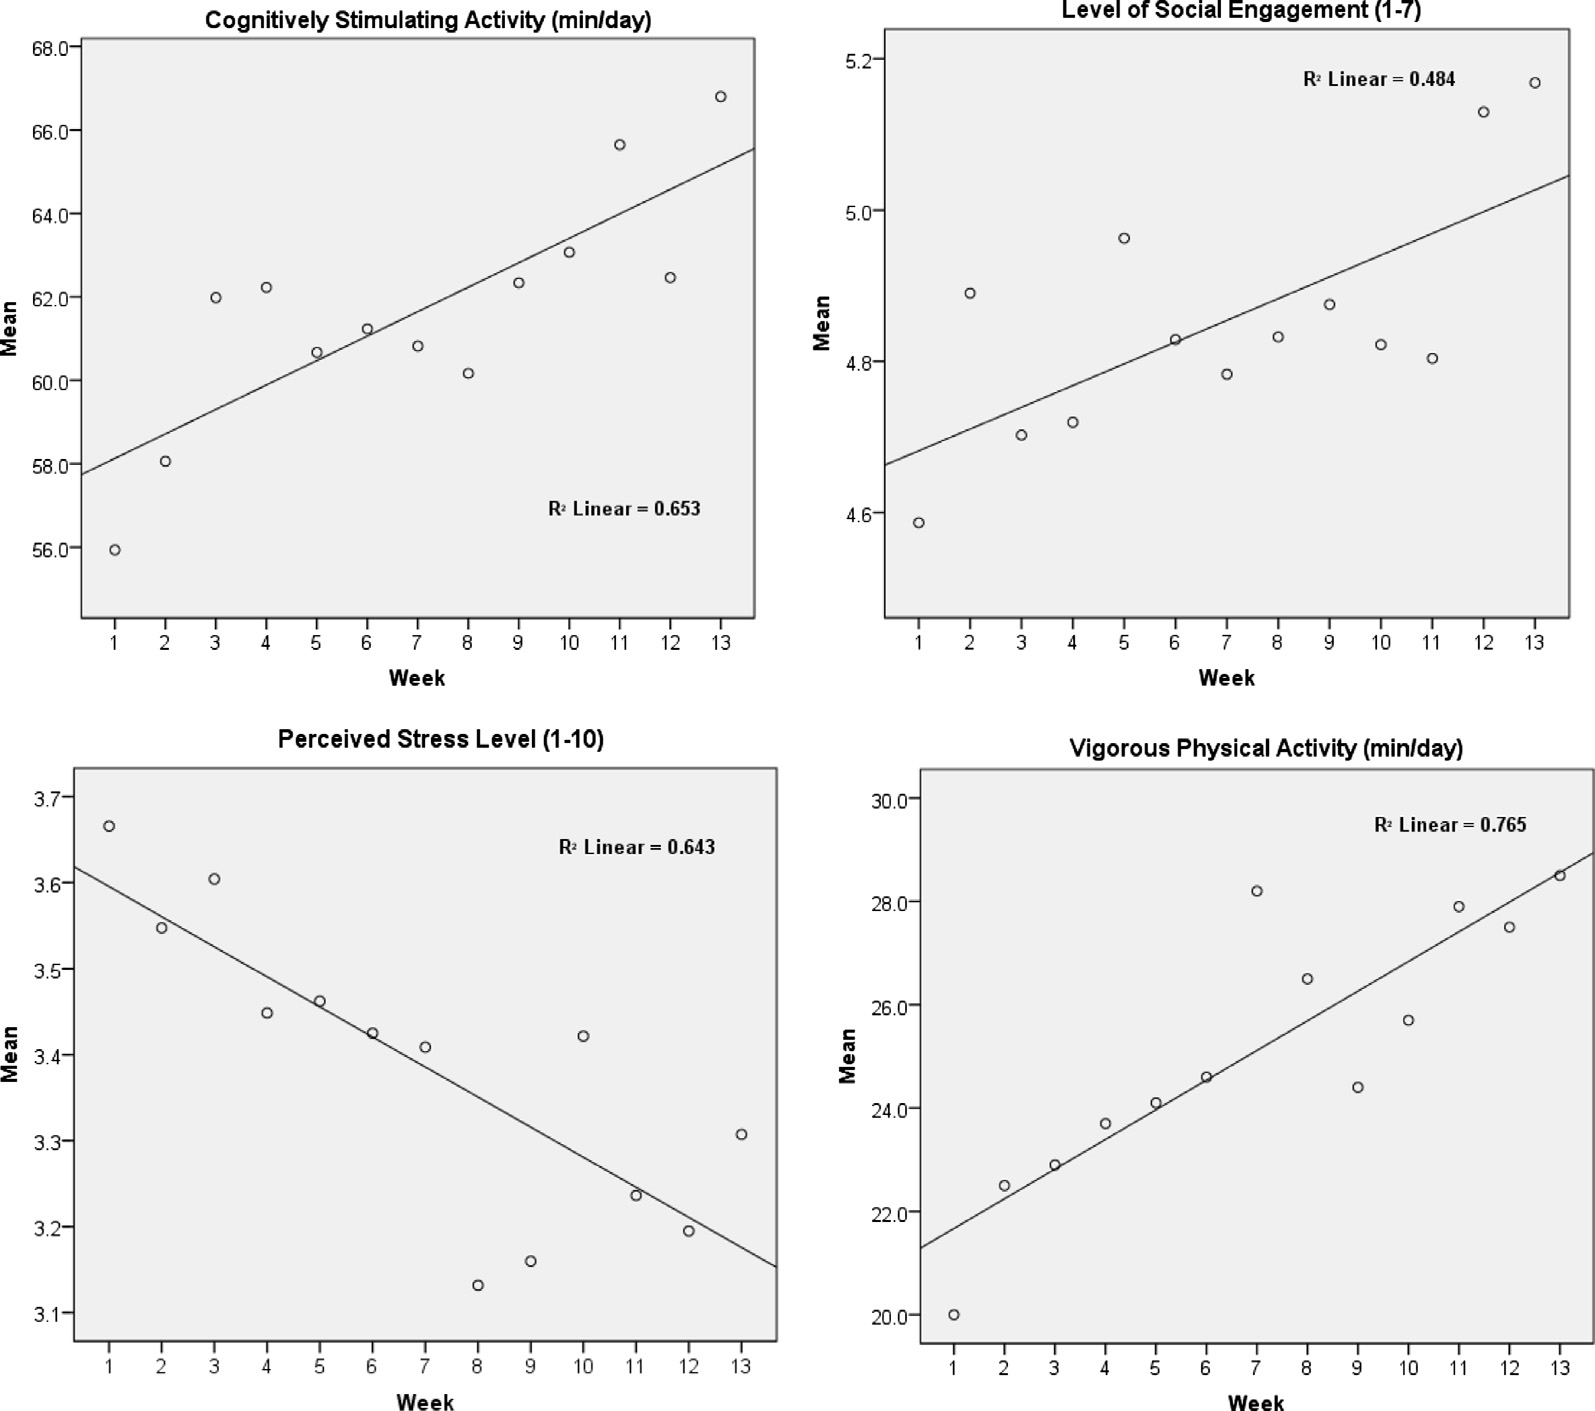
\includegraphics[scale=0.25, angle=0]{Files/prevention-study-3/figures/behaviourchange-week14}
    \caption{Weekly averages of four daily behavioural levels (averaging daily values within each week) for cognitively stimulating activities ($\beta$ = 0.81, p = .001), social engagement levels ($\beta$ = 0.70, p = .008), perceived stress levels ($\beta$ = 20.81, p = .001), and vigorous physical activity ($\beta$ = 0.88, p = .001); all coefficients are standardised.}
    \label{fig: preliminary-analysis}
\end{figure}

\subsection{Progression and Maintenance}
At the close of the study, it was possible to have a full picture of how each participants behaviour changed over the 26 week period.
To study this change at a high level, the mean performance of achieving the recommended values, across all domains, was calculated on a week-by-week basis for each participant. These individual values were then combined to establish the mean performance of the entire treatment cohort, for each week, across the 26 week period. To account for the varying levels of performance observed in the study, 2 forms of performance value were calculated for each log:

\begin{enumerate}[noitemsep,topsep=0pt]
\item Mean performance not accounting over-achievement; Performance max value fixed to 100\% (Limited).
\item Mean performance allowing for over-achievement; No fixed upper limit. (Not limited).
\end{enumerate}

\subsubsection{Correlation}
Bivariate correlation analysis showed a significant strong positive relationship between the week and mean performance in values which were limited (r = .832, p = \textless .000). There was also a significant strong positive relationship found between the week and mean performance in values which were not limited (r = .776, p = \textless .000).

\subsubsection{Linear Regression}
Linear regression analysis shows that the number of weeks using the app explain a significant amount of the variance in the performance scores, limited [F(1, 24) = 54.007, p = \textless.000, R\textsuperscript{2} = .692, R\textsuperscript{2}\textsubscript{Adjusted} = .68], and not limited [F(1, 24) = 36.402, p = \textless.000, R\textsuperscript{2} = .603, R\textsuperscript{2}\textsubscript{Adjusted} = .586], respectively. Visual plots of these regression lines can be seen in Figure \ref{fig: performance-linear-limitcomparison}.

\begin{figure}[h]
    \centering
    \begin{subfigure}[t]{0.48\textwidth}
        \centering
        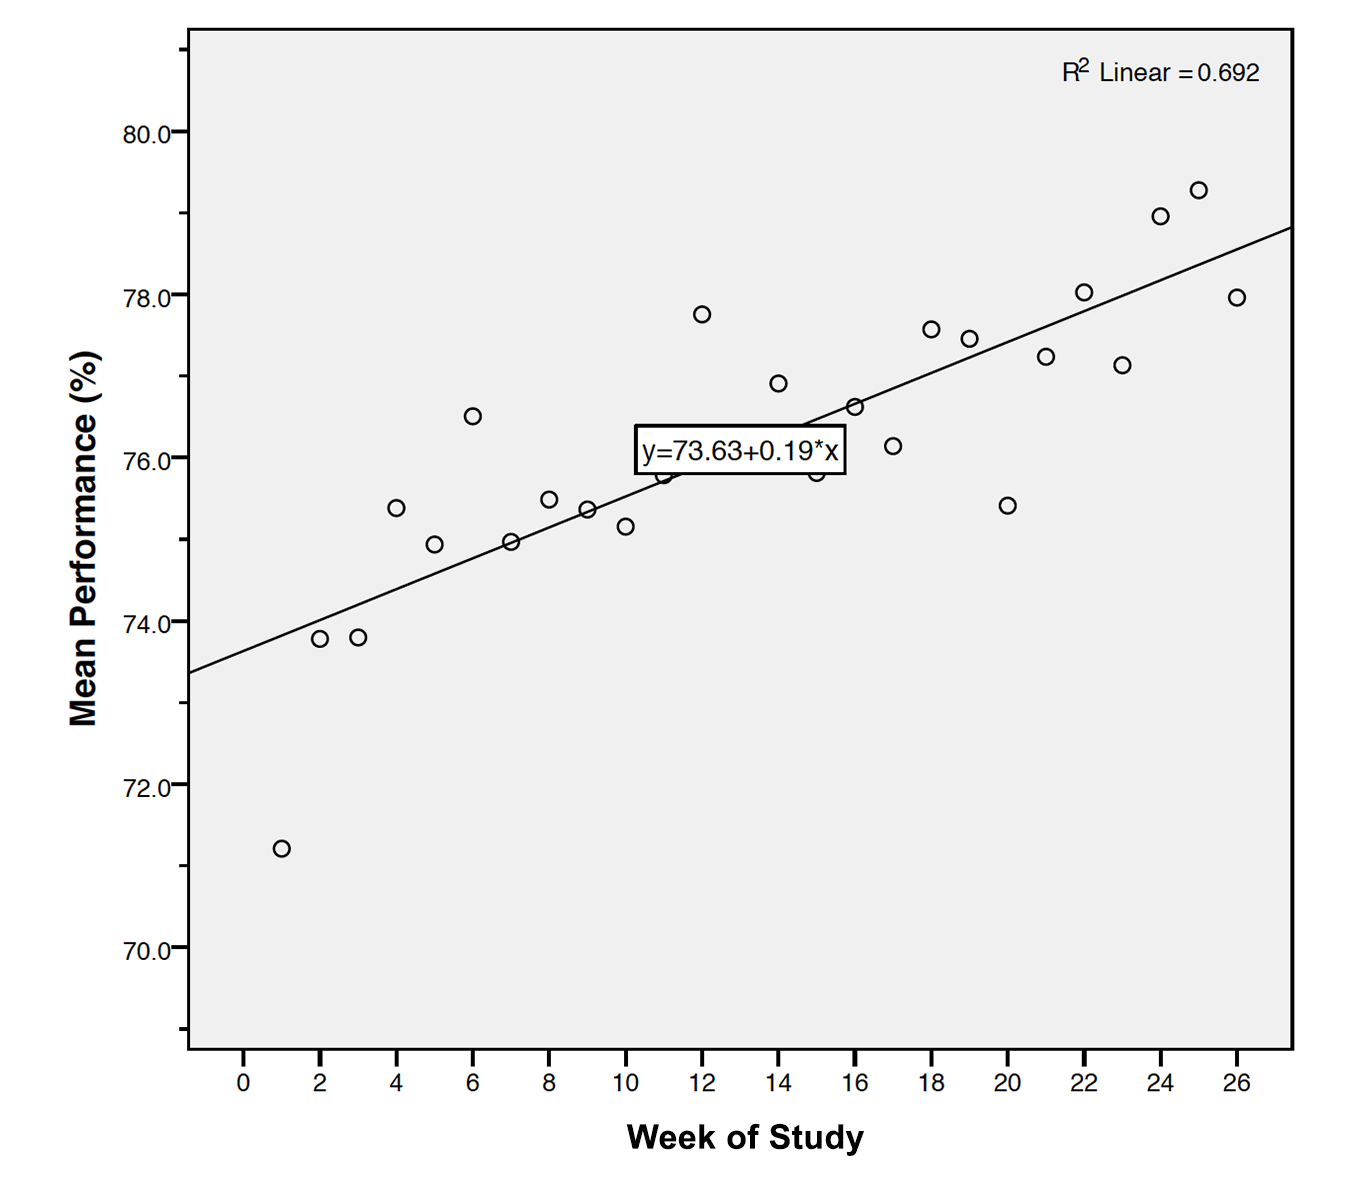
\includegraphics[width=\textwidth]{Files/prevention-study-3/figures/performance-linear-limit}
        \caption{Limited}
        \label{fig: performance-linear-limit}
    \end{subfigure}
    \hfill
    \begin{subfigure}[t]{0.48\textwidth}
        \centering
        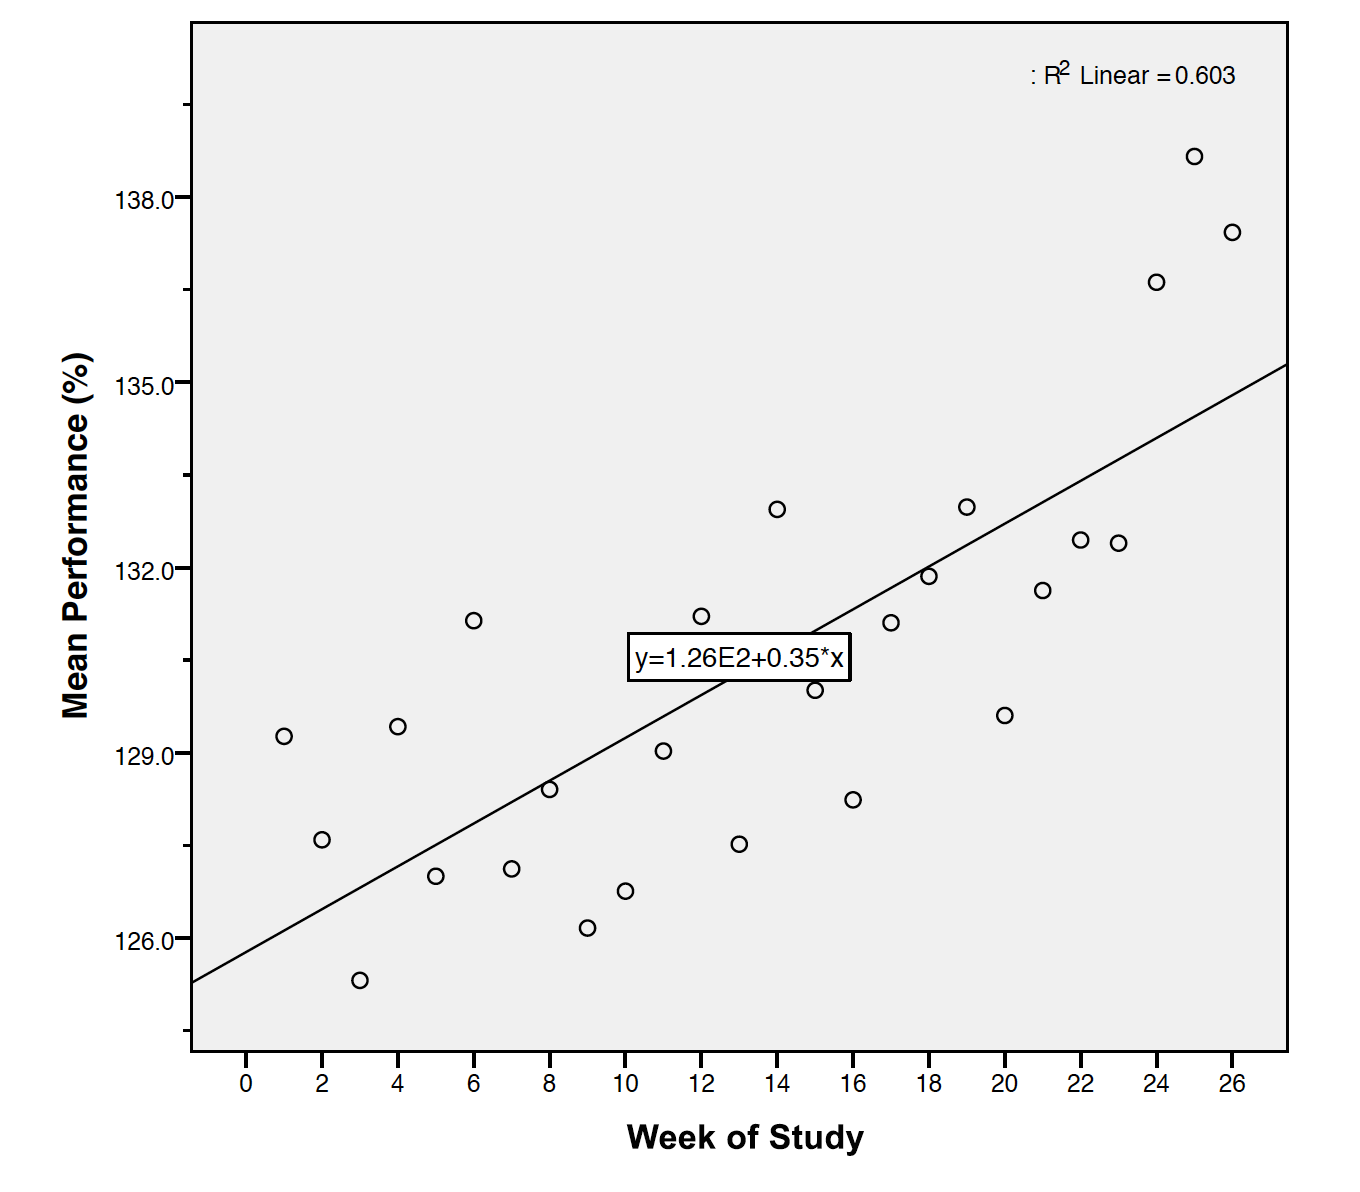
\includegraphics[width=\textwidth]{Files/prevention-study-3/figures/performance-linear-nolimit}
        \caption{No Limit}
        \label{fig: performance-linear-nolimit}
    \end{subfigure}
    \caption{Scatter plot showing performance scores (limited and not) against Week number with fitted linear regression lines}
    \label{fig: performance-linear-limitcomparison}
\end{figure}

\textbf{Limited variables.}
For each additional week, recommended guideline achievement performance increased by 0.189\%. The linear regression equation is as follows:
\begin{equation}
Performance = 73.63 + \left(0.189 \times Week\right)
          \label{eq: calc-performance-limited-behaviour-change}
\end{equation}

Using such a model, to achieve the full 100\% consistently, the participant would need to be actively engaged in the process for \textbf{139.523} weeks. Such an achievement is highly unrealistic, yet this model gives insight into the time and effort commitment required of persons seeking to positively change their behaviours.

\textbf{Not limited variables.}
For each additional week, recommended guideline achievement performance increased by 0.347\%. The linear regression equation is as follows:
\begin{equation}
Performance = 125.772 + \left(0.347 \times Week\right)
          \label{eq: calc-performance-notlimited-behaviour-change}
\end{equation}

Using such a model, to achieve 100\% consistently, the participant would need to be actively engaged in the process for \textbf{0} weeks. Obviously such a model is unrealistic and skewed, which exposes the issues arising from the use of scores which were not limited to 100\% in the analysis. The root of this issue lies with the variation measurement types used in the behavioural questions. Qualitative questions such as rating stress levels and social engagement, were within a fixed scale (E.g. 0-10), and as such it was impossible to `over-achieve' in these measures. Quantitative measures however, such as physical activity and dietary behaviours, allowed for the entry of values which were above the recommended levels, thus allowing participants to over-achieve. This unbalanced ability to over-achieve in certain domains, and not in others, greatly diminishes the use of any achievement percentages over 100\%. As such, only answers limited to 100\% are considered for further analysis.

\subsubsection{Non-linear regression}
Despite the significance found within correlation analysis (r = .832, p = \textless .000) and a good fit within linear regression (R\textsuperscript{2} = .603, p = \textless.000), behaviour change is a very individual process, during which levels of achievement are expected to peak, plateua, re-adjust, and improve again. Such changes can be seen in the observed data shown in Figure \ref{fig: performance-linear-limitcomparison}. As such, the relationship between the week, and level of achievement experienced may be non-linear, and so the linear regression model above may not be the best fit. Due to the changes observed in the data, in particular the observation of plateauing and subsequent improvement, cubic regression was identified as a possible means to model the data. A comparison of the linear and cubic regression lines fitted to the data can be seen in Figure \ref{fig: performance-cublic-linear-limited}.
 \begin{figure}[h]
    \centering
    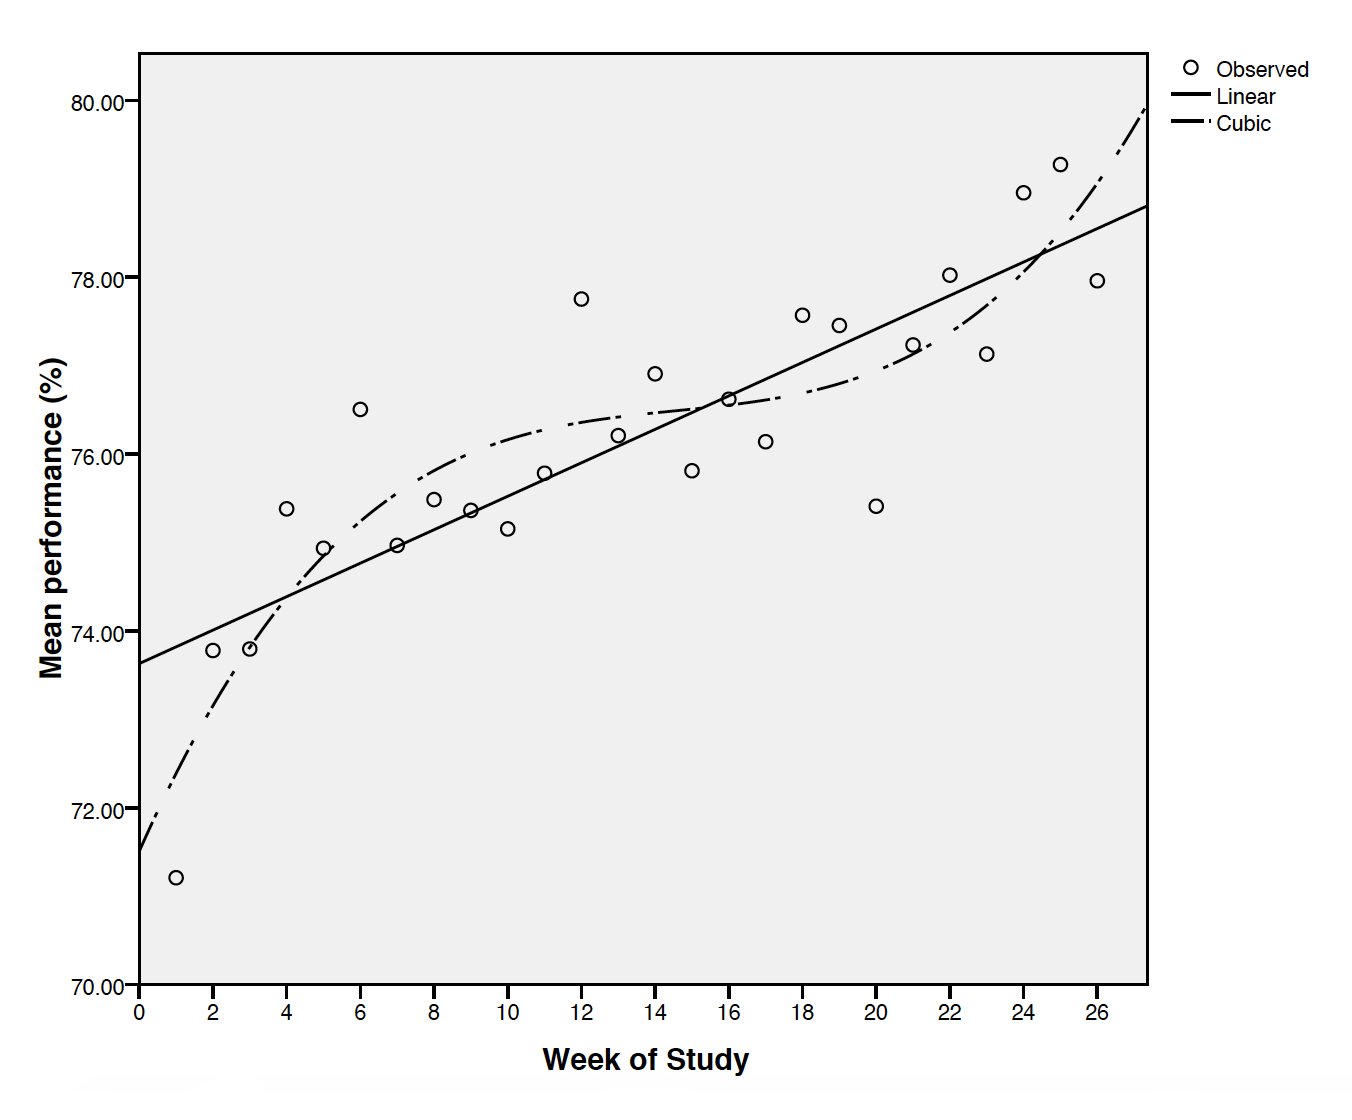
\includegraphics[scale=0.25, angle=0]{Files/prevention-study-3/figures/performance-cublic-linear-limited}
    \caption{Comparison of linear (R\textsuperscript{2} = .603, p = \textless.000) and cubic regression (R\textsuperscript{2} = .784, p = \textless.000) lines fitted to mean behaviour change observed over 26 weeks}
    \label{fig: performance-cublic-linear-limited}
\end{figure}
The cubic regression model provides a closer fit to the observed data [F(3, 22) = 26.671, p = \textless.000, R\textsuperscript{2} = .784, R\textsuperscript{2}\textsubscript{Adjusted} = .755], than the previous linear model. Within this model, the cubic regression equation is as follows:
\begin{equation}
Performance = \left(0.01 \times Week\right)^{3} +  \left(0.062 \times Week\right)^{2} +  \left(9.41 \times Week \right) +  71.508
          \label{eq: calc-performance-notlimited-behaviour-change}
\end{equation}

Using this equation, a participant is predicted to reach 100\% performance in achieving recommended behaviours related to AD risk for all domains in after approximately 40 weeks of effort. To achieve such a goal would be an impressive feat, as adherence to recommended guidelines is typically very low. In the United Kingdom only 35\% of men and 24\% of women achieve the recommended targets for moderate-intensity activity \cite{Miles2007}.

\subsection{Additional analysis}
During the analysis of behavioural data, it became apparent that certain internal components of the study, namely booster events, may of had an effect on behaviours, as did certain external factors \cite{Hartin2015-ICOST}.

\subsubsection{The effect of booster events}
To analyse the effect that booster events may have on behaviours, a list of events and attendees were analysed. For each attendee at an event, their log responses to the relevant domain questions were compared one week (7 days) prior and post attendance. A Paired-sample t-Test between pre-post attendance highlighted a significant change at the p \textless 0.05 level in domain relevant behaviours for 7 of the 46 events \cite{Hartin2015-ICOST}. Additional detail of these 7 events, including event titles, domains, descriptive statistics of relevant behaviours can be seen in Table \ref{tbl: booster-significance}. It must be noted that not all booster events had the desired effect in the observed short term. For example, attendees of events 4 and 15, reported significantly less effort and activity after attending the booster events. For these cases it may be assumed that the attendees felt they overachieved in these areas through attending the event, and reduced their conscious efforts in the following week. Further work is required to test this assumption.

\begin{sidewaystable}
\centering
\caption{List of booster events which resulted in a significant difference in behaviours after attendance.}
\label{tbl: booster-significance}
\resizebox{\textwidth}{!}{%
\begin{tabular}{@{}llllllllll@{}}
\toprule
Event ID \# & Booster Event Activity & Domain & Question & \begin{tabular}[c]{@{}l@{}}Mean \\ (Pre)\end{tabular} & \begin{tabular}[c]{@{}l@{}}Mean \\ (Post)\end{tabular} & \begin{tabular}[c]{@{}l@{}}Std. Dev \\ (Pre)\end{tabular} & \begin{tabular}[c]{@{}l@{}}Std. Dev \\ (Post)\end{tabular} & \begin{tabular}[c]{@{}l@{}}Sig.\\ (2-Tailed)\end{tabular} & \begin{tabular}[c]{@{}l@{}}Num.\\ Attendees\end{tabular} \\ \midrule
4 & Mindfulness & Stress & Self effort to decrease stress & 4.43 & 5.73 & 2.10 & 1.63 & 0.03 & 5 \\
15 & Learning to paint & Mental & Cognitively stimulating activity (mins) & 73.67 & 64.52 & 28.83 & 24.06 & 0.03 & 11 \\
24 & Intro to  Pilates & Physical & Vigorous physical activity (mins) & 24.69 & 25.88 & 16.81 & 13.39 & 0.046 & 9 \\
25 & Pilates Reformer & Physical & Moderate physical activity (mins) & 41.25 & 43.11 & 2.84 & 19.11 & 0.021 & 3 \\
29 & Yummy dips for fresh veggies & Food & Fruits and veg consumption (cups) & 3.63 & 4.49 & 1.24 & 1.39 & 0.038 & 6 \\
33 & Relationship Enrichment & Social & Self-rate stress level & 3.03 & 2.38 & 1.91 & 1.28 & 0.03 & 10 \\
36 & Salads and Stir-fry & Food & Nuts, seeds, or legumes consumption (cups) & 1.32 & 1.68 & 0.68 & 0.87 & 0.029 & 7 \\ \bottomrule
\end{tabular}}
\end{sidewaystable}

\subsubsection{The effect of weather conditions}
In addition to internal study components, a number of external factors were also analysed for effect, such as public holidays and local weather conditions.
Analysis of local weather conditions resulted in a finding of positive correlation between local temperature in the Cache County area with physical activity, both moderate and vigorous, R = 0.585, R = 0.725, respectively \cite{Hartin2015-ICOST}. Figure \ref{fig: scatter-regression-temp-activity} shows that as local temperature increases, vigorous physical activity also increases.

\begin{figure}[h]
    \centering
    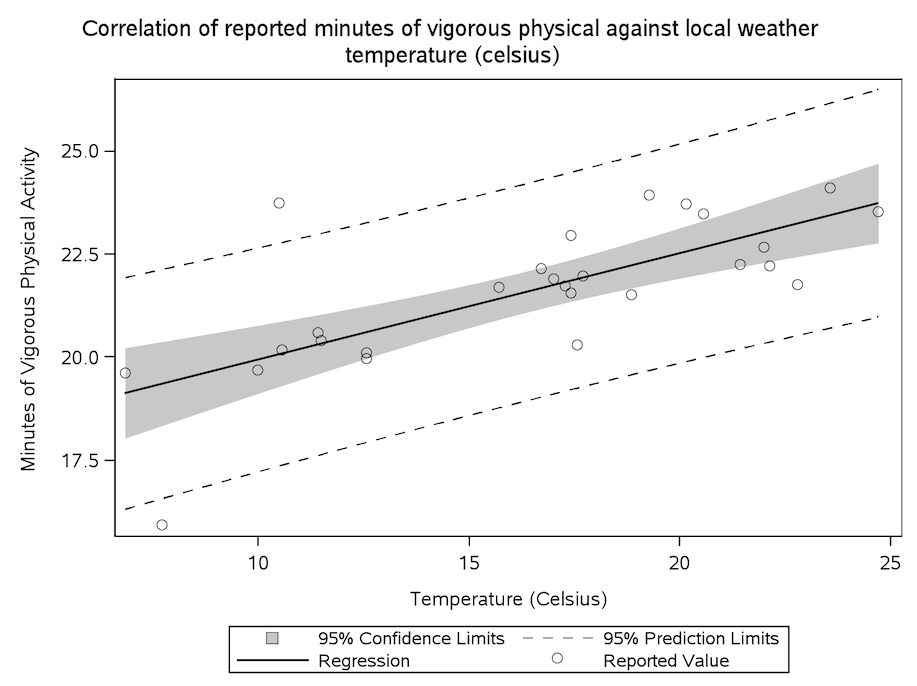
\includegraphics[scale=0.4, angle=0]{Files/prevention-study-3/figures/correlation-temp-activity}
    \caption{Scatter plot showing correlation analysis of participant’s self-reported vigorous exercise against the external factor local average temperature in degrees Celsius (R = 0.725, p = \textless.0001)}
    \label{fig: scatter-regression-temp-activity}
\end{figure}


\section{Clinical Outcomes}
Whilst behaviour change was shown to occur within individuals in the study, the effect on their health outcomes must still be determined. As shown in Table \ref{tbl: clinical-variables}, a number of biological and clinical markers were taken from each participant at the beginning and end of the study. This data has been processed and analysed for trends and correlations. In addition, this clinical data has also been paired with the previously discussed app usage and behavioural datasets, from which a number of hypothesises are developed and tested.

\subsection{Number of times app used per week}
Logically, it is hypothesised that increased exposure to the app and its material would result in favourable outcomes, both in behaviour change and in clinical markers.
\subsubsection{Method}
Firstly, the number of times that the app was launched per week was established and categorised into groups (\textless1, 1-3, 3-5, 5-7, 7+ per week). These groups were then evaluated with various clinical and biometric measurements taken from the participants at the start and end of the study, along with the control group.
\subsubsection{Results}
From a high-level, it is evident that increased app exposure has an observable effect in various clinical measurements, with particularly observable effects within BMI and systolic blood pressure (SBP) measurements, shown in Figure \ref{fig: applaunch-bmi} and Figure \ref{fig: applaunch-bp}, respectively.

\begin{figure}[h]
	\centering
    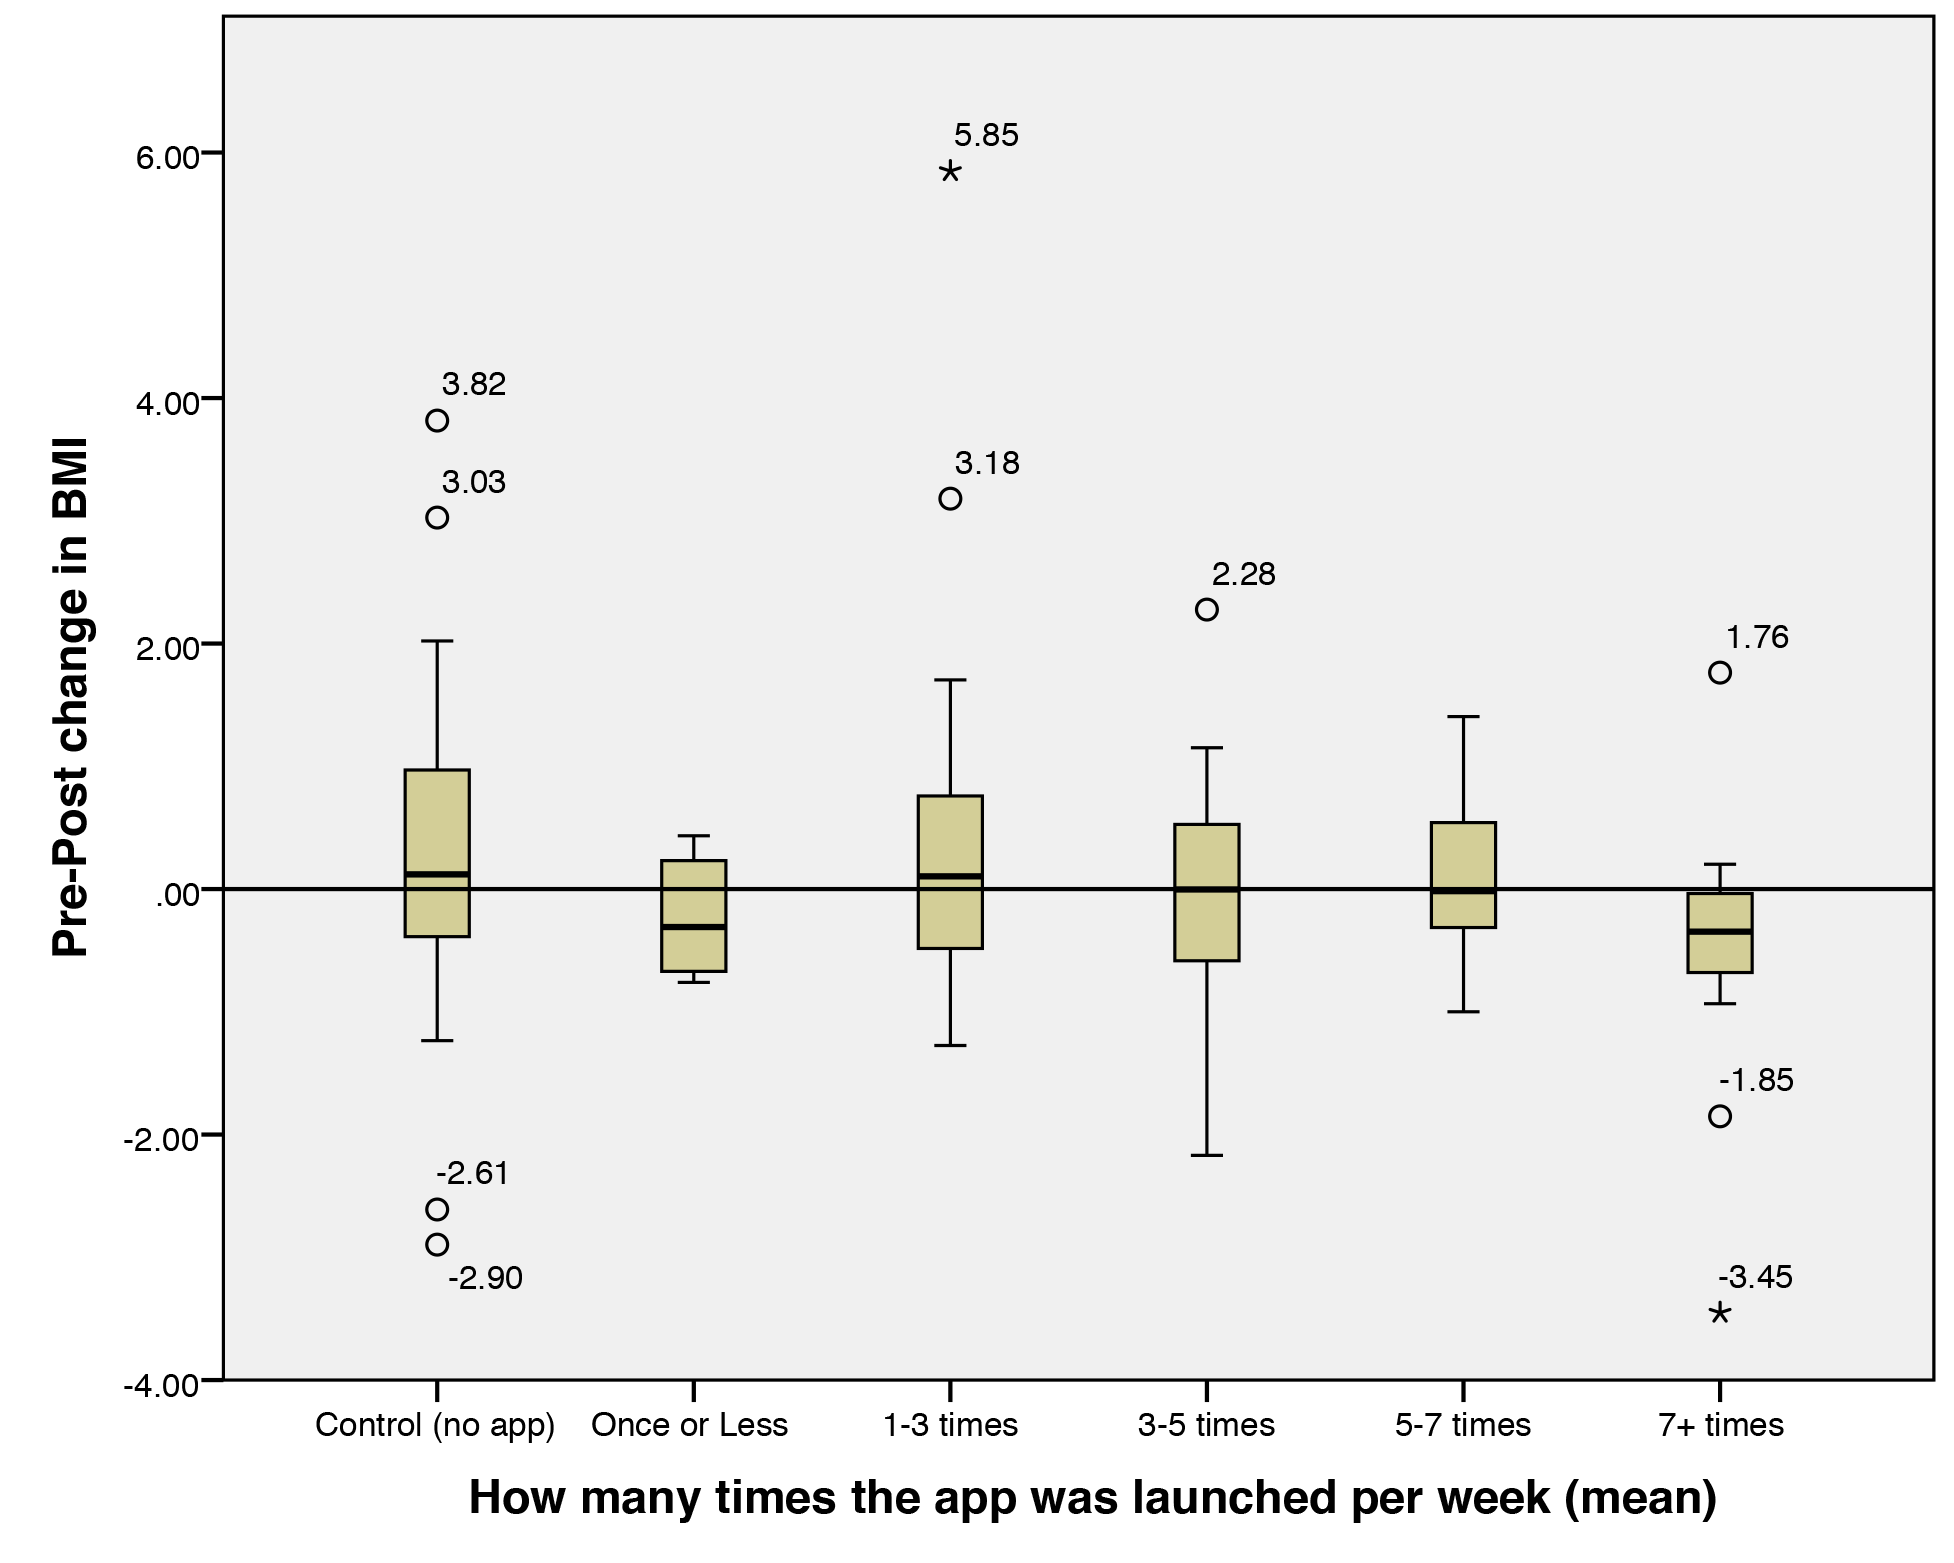
\includegraphics[scale=0.18, angle=0]{Files/prevention-study-3/figures/applaunch-bmi}
  	\caption{Boxplot showing no app (control) and grouped app launches per week (treatment) against observed changes in BMI. Outliers are plotted as individual points.}
    \label{fig: applaunch-bmi}
\end{figure}

\begin{figure}[h]
	\centering
    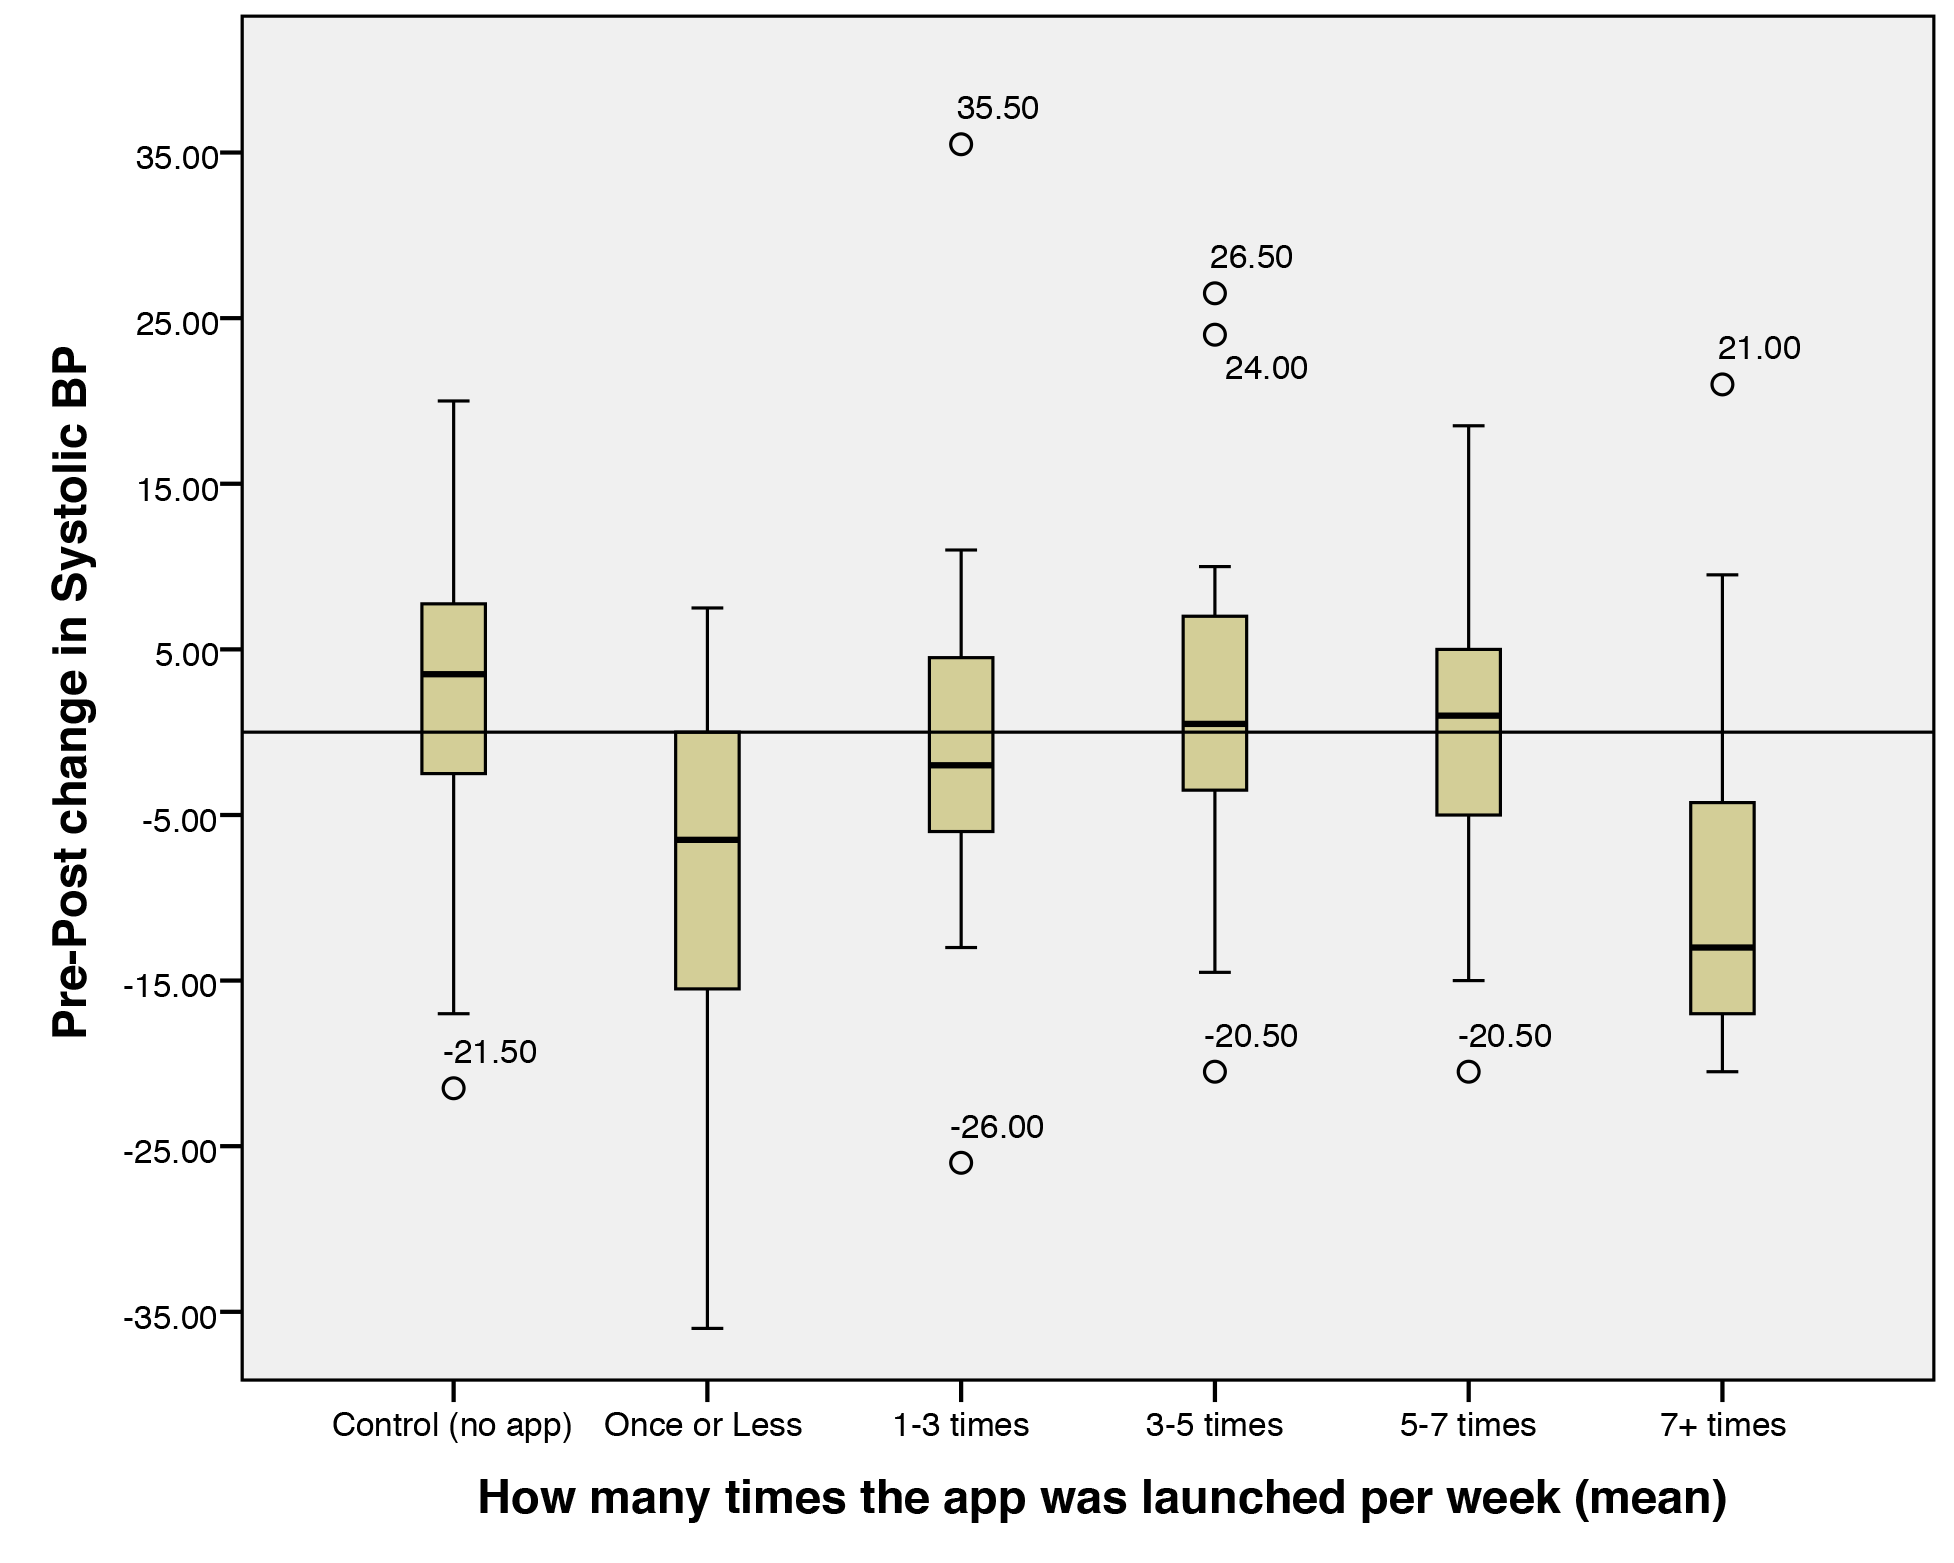
\includegraphics[scale=0.18, angle=0]{Files/prevention-study-3/figures/applaunch-bp}
  	\caption{Boxplot showing no app (control) and grouped app launches per week (treatment) against observed changes in systolic blood pressure (mm/Hg). Outliers are plotted as individual points.}
    \label{fig: applaunch-bp}
\end{figure}

It can be seen that the control group have undesirable increases over the intervention period, whilst the treatment group have sustained or reduced their measurements. Notably, those who looked at the app \textit{greater than 7 times per week} appear to have the largest reduction in BMI and blood pressure, whilst those less than 7 times and greater than 1 vary in their results \cite{Hartin2015-JMIR}. It is also interesting to note that those who looked at the app once or less per week also maintained favourable rates of decline. It is proposed that these users are self-sufficient in their efforts to enact behaviour change and do not require the app to aid them.

\subsection{Compliance to log-entry}
The average number of logs completed per day were analysed for correlations to the clinical changes observed in the study, suggesting the following hypothesis:
\begin{description}
  \item[H1] The number of logs completed each day will correspond to greater change in clinical and biological markers.
  \item[H0] There is no supported relationship between daily log and clinical or biological markers.
\end{description}

\subsubsection{Method}
The clinical measurements were analysed as both their raw values, as continuous variables, and also as dichotomous groups. These groups were classes as showing Improvement or No Improvement post intervention, made possible using domain knowledge.

\subsubsection{Results}

\textbf{Continuous Variables.}
Analysis shows that daily log completion rates show no relationship between pre-post BMI scores (r = .016, p = .872) and diastolic blood pressure (r = .064, p = .523). There is a weak positive correlation found in systolic blood pressure (r = .28, p = .784), and weak negative relationships in resting heart-rate (r = -.121, p = .23) and blood carotenoids (r = -.105, p = .294). Further correlation analysis was completed on the biological markers, which also showed positive, but weak, correlation between the number of logs completed and pre-post total cholesterol (r = .145, p = .91) and triglycerides (r = .145, p = .15), and negative, weak, correlation in serum glucose (r = -.88, p = .382) and blood insulin levels (r = -.105, p = .296).
Nevertheless, calculating partial correlation, controlling for the number of days the participant had the app installed, highlighted toward a significant correlation between total cholesterol and average questions per day (r = .193, p = .055). Adding an extra control for the participant’s initial recorded total cholesterol levels resulted in a significant correlation (r = .228, p = .024). We therefore reject the null hypothesis for this particular case.

\textbf{Dichotomous Groups.}
After categorising pre-post results as showing improvement, or not improvement, independent samples t-Tests showed that participants who improved their HDL cholesterol levels during the study duration answered a statistically significant higher number of questions per day (8.30 $\pm$ 2.29) than those with no improvement (6.52 $\pm$ 3.612), t(97.74) = -3.051, p = .003.

\subsection{Achieving recommended daily targets}
As one of the primary methods by which participants were educated about favourable lifestyle behaviours, the recommended daily targets served an important function. In addition, these targets were established using the latest scientific literature. To evaluate the effect of achieving these targets the following hypothesis is tested:
\begin{description}
  \item[H1] The greater number of recommended goals achieved, the larger the degree of change in clinical and biological markers.
  \item[H0] There is no supported relationship between achieving recommended values and clinical or biological markers.
\end{description}

\subsubsection{Method}
Participants’ self-reported behaviours were analysed to find the frequency and percentage of times that they achieved the recommended daily goal value for each question. Once again, in addition to these continuous measures, each pre-post clinical and biological reading was categorised into groups, showing Improvement or No-Improvement.

\subsubsection{Results}
\textbf{Continuous Variables.}
Correlation analysis between a participant’s mean percentage of recommended goals achieved, across the study duration, and observed clinical measurement changes showed the following: No relationship for systolic (r = -.013, p = .896) and diastolic (r = -.35, p = .732) blood pressures, and no relationship in carotenoids (r = -.013, p = .895). Positive, but weak, correlation was found in resting heart rate (r = -.107, p = .285) and also BMI change (r = .157, p = .116). Biomarker changes were also correlated against percentage of recommended values achieved showing: No correlation in serum glucose (r = -.075, p = .455) and blood insulin levels (r = -.049, p = .624). Positive, but weak, correlation was found for pre-post triglyceride values (r = .155, p = .124). Significant correlation, at the 95\% confidence interval, was found in pre-post total cholesterol (r = .217, p = .03). The null hypothesis is accepted for all but this case.

\textbf{Dichotomous Groups.}
For each individual, a base-line performance level was calculated from their self-reported behaviours in their first week of enrolment. Since there were a number of highly active and healthy living individuals within the treatment group, to reduce the ceiling effect on the data, the first quintile (n=20) of participants were removed from the analysis. Using the dichotomous groupings of Improvement and No-Improvement, significant correlations were found between daily goal percentage achieved and BMI reduction (r = .264, p = .017). An independent samples t-Test showed participants who decreased their BMI achieved a significantly higher percentage of attaining attaining their recommended daily goals (56.21 $\pm$ 30.4\%) than those who increased their BMI (40.12 $\pm$ 29.1\%), t(80) = -2.449, p = .017. Further analysis showed that 69.2\% (n=18) of those who achieved a mean performance percentage of 60\% or greater, across all domains, reduced their BMI during the study, whereas 60.7\% (n=34) of those who did not, increased their BMI.

\begin{table}[h]
\centering
\caption{Odds ratio and relative risk analysis for participants who achieved over 60\% of their recommended daily targets (mean) and BMI change outcome.}
\label{tbl: oddsratio-recommendedtargets-bmi}
\begin{tabular}{@{}llll@{}}
\toprule
\multirow{2}{*}{} & \multirow{2}{*}{Value} & \multicolumn{2}{l}{95\% CI for Mean} \\ \cmidrule(l){3-4}
 &  & Lower & Upper \\ \midrule
\begin{tabular}[c]{@{}l@{}}Odds Ratio for Recommended Achieved \textgreater60\% \\ (Achieved / Did Not Achieve)\end{tabular} & .288 & .107 & .774 \\
For cohort BMI change = Increased & .507 & .274 & .936 \\
For cohort BMI change = Decreased & 1.762 & 1.164 & 2.667 \\
N of Valid Cases & 82 &  &  \\ \bottomrule
\end{tabular}
\end{table}

Analysis of cross tabulation, displayed in Table \ref{tbl: oddsratio-recommendedtargets-bmi}, shows that those who achieved over 60\% of their recommended daily goals were 1.762 times more likely to decrease their BMI during the study, or 0.507 times less likely to increase their BMI, than those who did not achieve 60\%.

\subsection{Physical activity levels}
Physical activity levels were assessed in the study through the participants self-reported behaviours in the following 3 questions:
\begin{enumerate}[noitemsep,topsep=0pt]
	\item Number of minutes performing moderate physical activity
	\item Number of minutes performing vigorous physical activity
	\item Nike fuel points earned via wearable device
\end{enumerate}

Each participant’s results were analysed for correlations between these values and clinical observations. The following hypothesis is tested:
\begin{description}
  \item[H1] The greater number of minutes performing physical activity or greater number of fuel points achieved, the larger the degree of change in clinical and biological markers.
  \item[H0] There is no supported relationship between physical activity levels and/or fuel points with clinical or biological markers.
  \end{description}

\subsubsection{Method}
Participant's self-reported behaviours in the questions relating to physical activity were analysed. Changes in clinical and biological markers between pre and post intervention, were once again categorised as either showing improvement or no-improvement.
Again, using the base-line performance metric calculated on the first week of observation, participants in the last decile (bottom 10\%) were excluded from the analysis to reduce ceiling effects.

\subsubsection{Results}
\textbf{Vigorous activity.}
After removal of last decile, an independent samples t-Test found that the remaining participants (n=92) who decreased their BMI (n=45) reported statistically significantly more vigorous physical activity (23.94 $\pm$ 10.76 minutes) than those who increased their BMI (19.09 $\pm$ 12.36 minutes), t(90) = 2.002, p = .048.
\newline \textbf{Moderate activity.}
Interestingly no correlation was found with moderate physical activity levels and BMI reduction status.
\newline \textbf{Wrist-worn Wearable.}
Again no correlation was found with the number of fuelpoints achieved from the wrist-worn wearable device and BMI reduction status.
However, upon removing the first quintile, it was uncovered that those who improved their levels of HDL cholesterol during the intervention achieved significantly higher fuelpoints on a daily basis (2569.39 $\pm$ 641.17), than those who observed no improvement (2233.9 $\pm$ 800.34), f(82) = -2.052, p = .043. Literature in the area of endocrinology and metabolism supports this observation as physical exercise is associated with increases in HDL \cite{Franklin2014}.

\subsection{Stress reduction}
Within the literature, stress and its associated physiological resultants are considered valid components of AD risk \cite{Dotson2010,Royall2012,Boyle2010}. As hypertension is present in all major causes of cognitive impairment \cite{Iadecola2014}, it is of particular interest as a measurement when associated with stress and AD risk. As such participants’ self-reported stress reduction efforts were analysed for their effect on clinical measures, with specific emphasis on SBP.

\subsubsection{Methods}
Each participant’s SBP were recorded pre and post intervention and categorised into: Low (\textless90), Ideal (90-120), Pre-Hypertension (120-140) and Hypertension (\textgreater140). Those with non-ideal SBP at their pre-intervention recording (n=50) were analysed to observe if a change of category occurred during the intervention. Changes observed in these participants were categorised into 3 groups: Improvement (n=13), No-Improvement (n=14) or Deterioration (n=23).

\subsubsection{Results}
One-Way ANOVA analysis of their category changes showed a significant correlation between efforts to reduce stress (effort rated 1-10: 10 is high effort) and SBP category change as a whole, p = .035 (excluding first quintile of baseline performers). Multiple comparisons of the three groups showed significance between those who had no improvement (3.11 $\pm$ 2.32 effort rating) and those who had deteriorated (5.28 $\pm$ 2.105 effort rating), p = .028. No significant difference was found between improvement (4.18 $\pm$ 1.89 effort rating) and the remaining groups.

\subsection{Demographic Comparisons}
To fully utilise all available data, demographic information was also considered for analysis. To compare overall performance for participants during the study, the \textit{percentage of recommended values achieved} was used as the base metric. In addition, for the entire treatment cohort, each participant was categorised into quintiles based on their percentage of recommended values achieved (1=Highest, 5=Lowest). These performance quintiles were also then compared to a number of demographic variables collected at the start of the study.

\subsubsection{Family History of Alzheimer's Disease}
Analysis of this data showed relationships between a participant’s achieved percentages and if that participant knew of a member of their family having dementia. This relationship is especially when excluding the 1st quintile, and can be seen visually between the 2nd and 5th quintiles in \ref{fig: family-quintile}. The pattern observed shows that more participants who know of a family member with dementia achieve higher percentages of their recommended values than those who do not. Partial correlation within these quintiles, controlling for number of days enrolled in the study shows significant correlation (r = .232, p = .036).

\begin{figure}[h]
	\centering
    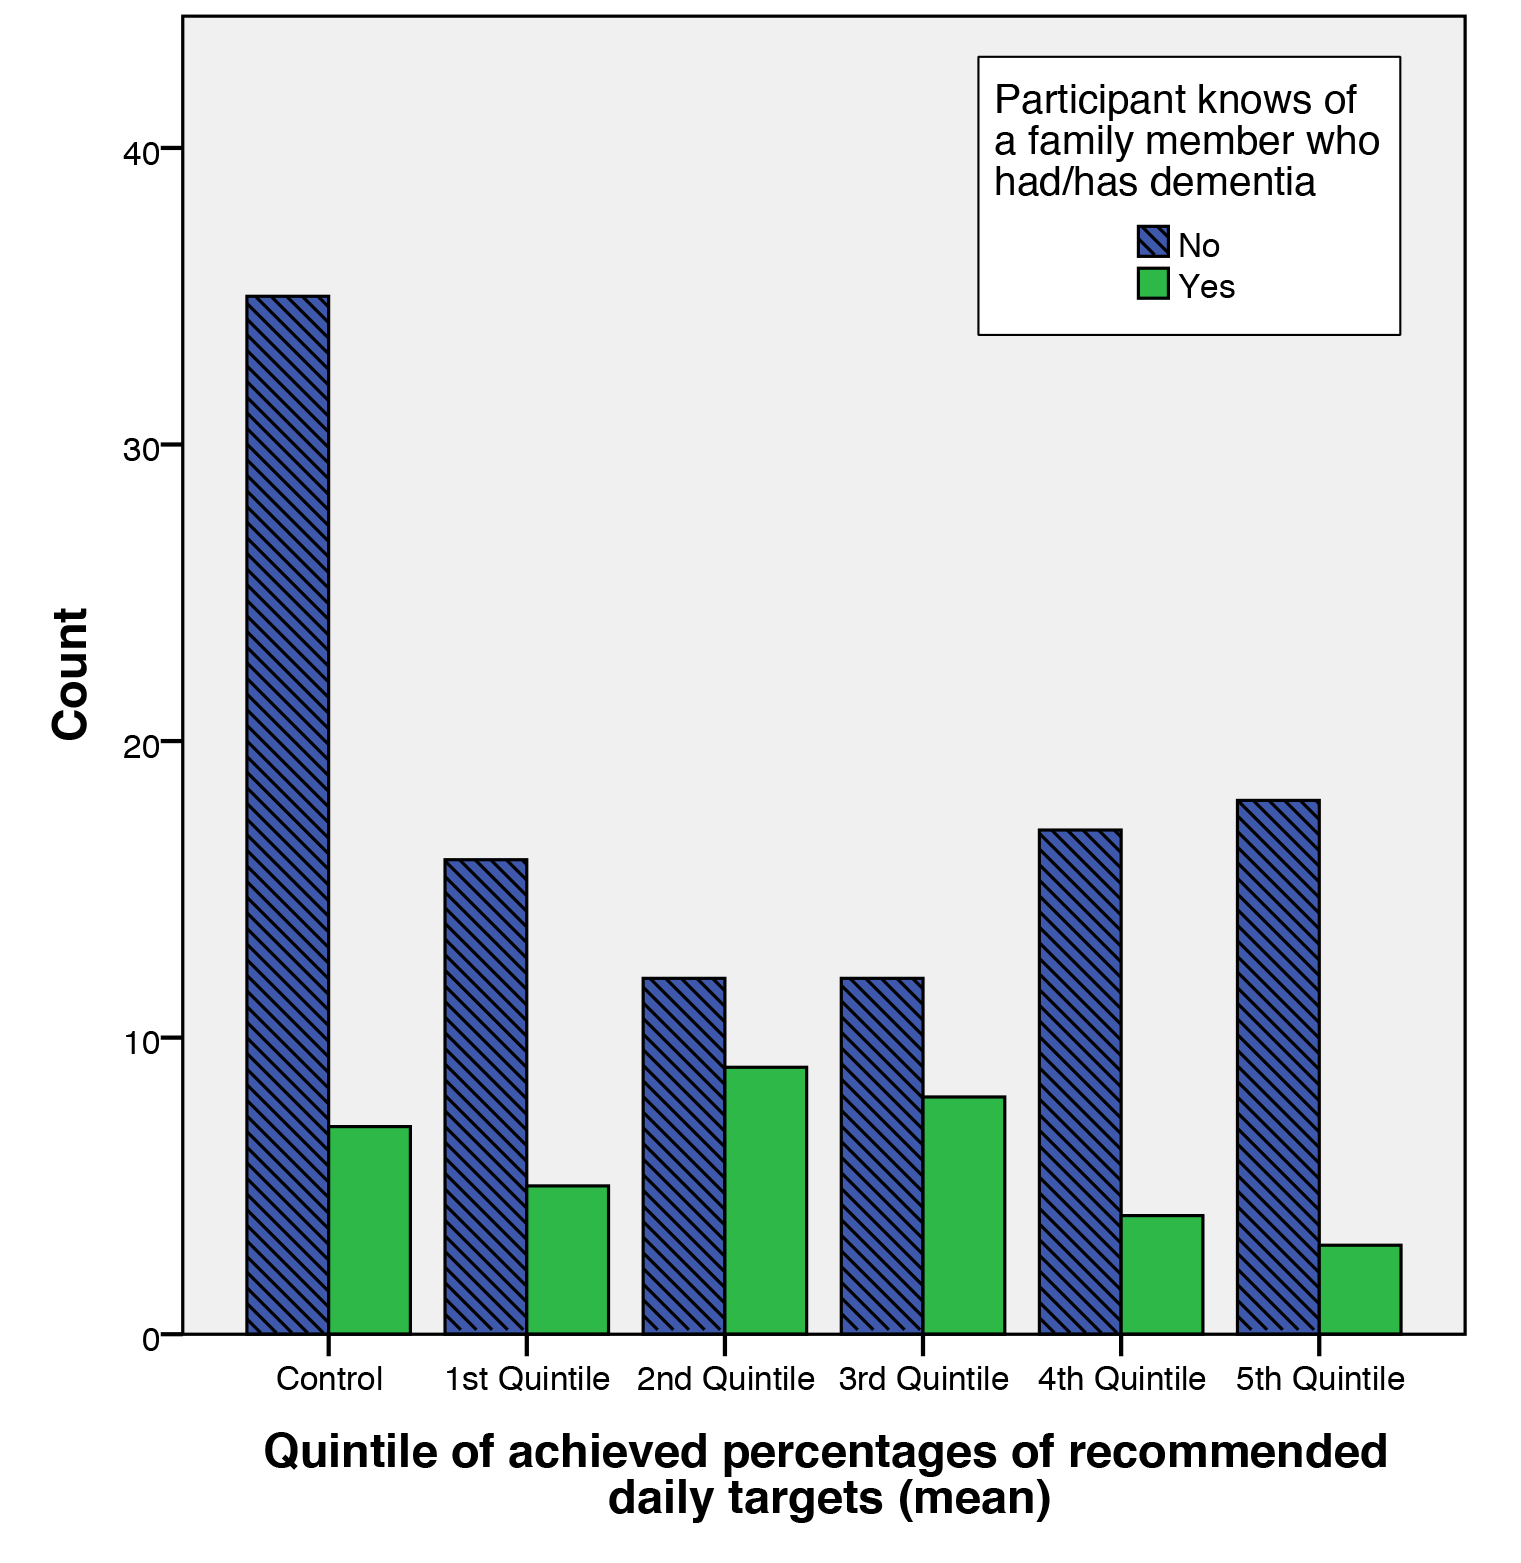
\includegraphics[scale=0.18, angle=0]{Files/prevention-study-3/figures/family-quintile}
  	\caption{Bar chart showing the performance quintiles and control group against the number of users who report to have known of a family member having/had dementia.}
    \label{fig: family-quintile}
\end{figure}

Research focused on the family members of persons with dementia has found that those who facilitate care typically suffer from higher rates of anxiety and depressive symptoms \cite{Mahoney2005}, and as such may be increasingly motivated to reduce their own risk. This behaviour seems to appear in this RCT, as participants in the treatment group who have members of family with dementia, and first-hand experience with the disease, are achieving a higher number of their recommended daily targets i.e. performing better within the realms of the study and theoretically reducing their AD risk.

\subsubsection{Gender}
As existing research has indicated that gender may play a role as to how AD risk is perceived or experienced \cite{Rose-Rego1998, Thompson2004}. As such the gender of participants and their achieved percentages were also analysed. Independent samples t-Test displayed that females achieved a statistically significant higher percentage of recommended targets (52.44 $\pm$ 29.24), compared to their male counterparts (38.69 $\pm$ 28.50), t(102) = -2.302, p = .023). In addition, analysis shows a visible correlation between gender and the ability to reach the recommended daily target values, as shown in Figure \ref{fig: gender-performance}. The reasons behind this particular observation are currently unclear and require additional analysis, however, could relate to motivations, occupation and education levels.

\begin{figure}[h]
	\centering
    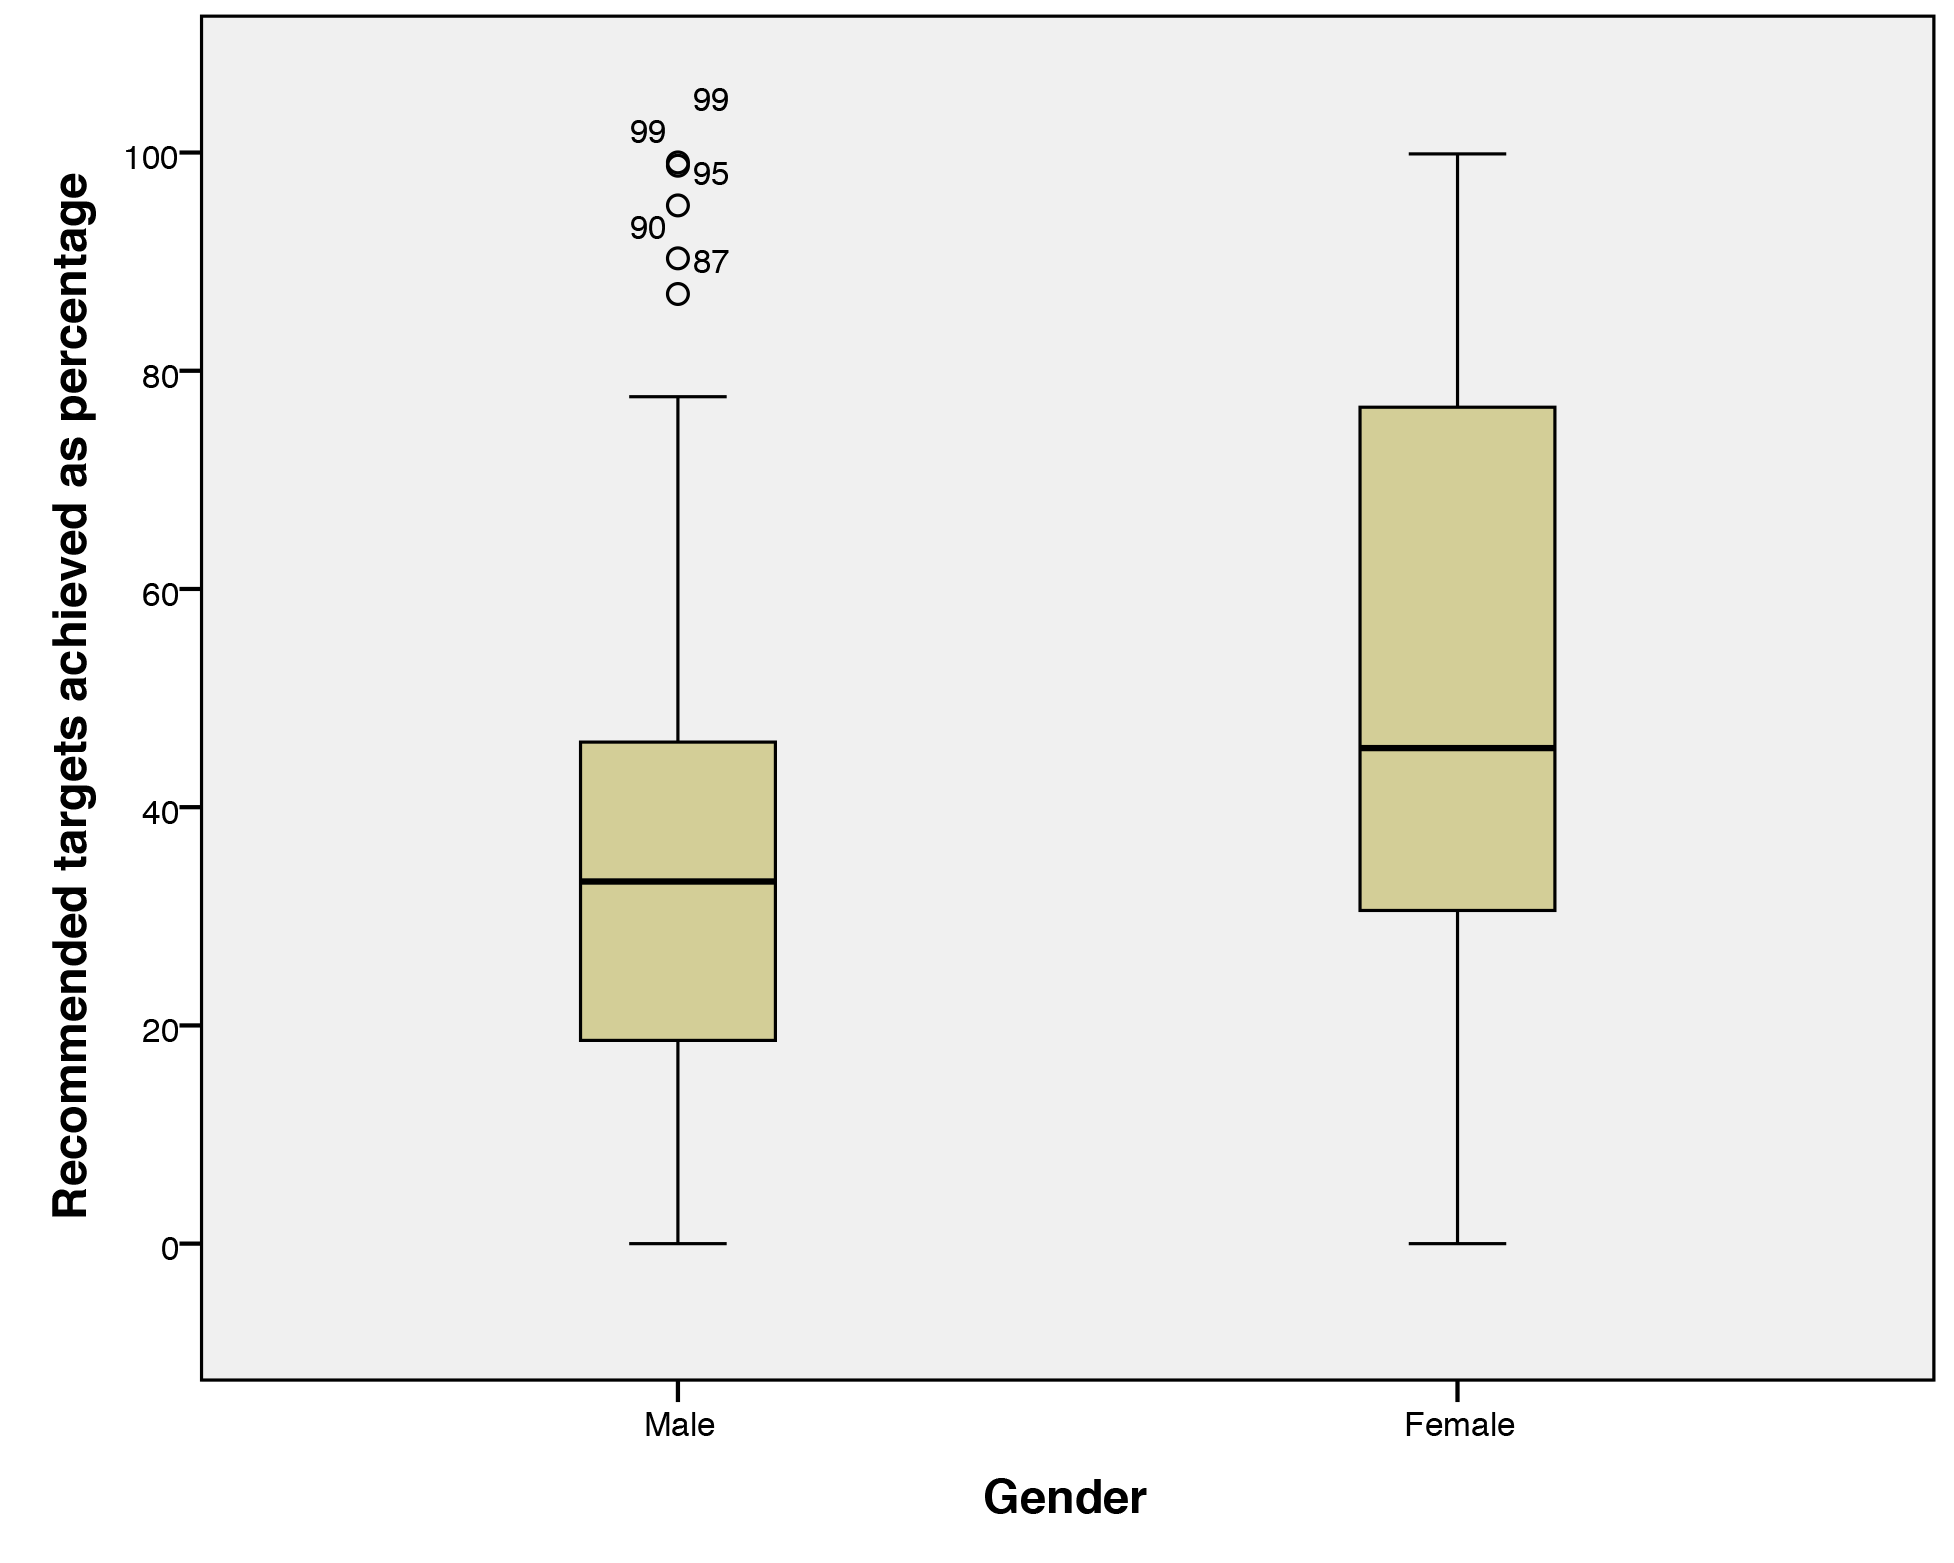
\includegraphics[scale=0.14, angle=0]{Files/prevention-study-3/figures/gender-performance.png}
  	\caption{Box-plot showing distributions of Male and Female mean percentages achieved targets across all domains.}
    \label{fig: gender-performance}
\end{figure}

\section{Principal Findings}
From the data generated within the RCT a number of results were found and have been categorised and presented, from a focal point of the smartphone app, as the principal findings of the study.

\subsection{Intervention delivery method}
The smartphone app provided a novel method to remotely monitor participants in a behaviour change intervention, whilst also facilitating the delivery of intervention material. The app had the ability to deliver multiple services through a single platform, and as a result was capable of facilitating stages 3-5 of the TTM, preparing participants for change, allowing them to accurately monitor and assess their actions and encouraging continued maintenance and improvement of their desired behaviours.
In addition, positive results from the exit-survey show that the majority of users wished to continue their behaviour change efforts, which were promoted by the app, and if maintained, are expected to yield superior outcomes in AD prevention.

\subsection{Importance of Goals and Recommended values}
In this trial, the recommended values for each behaviour played a key role in both motivating the participant's to change their behaviours, and also as a metric for the uniform assessment of participants’ performance. Analysis of pre-post measurements from the treatment group showed clear physiological changes in those who achieved the highest in their attempts to meet recommended values. This was especially apparent in those who were previously underachievers in certain behavioural domains, prior to the study (based on first week of observed behaviour logs). Effects observed included a desirable lowering of BMI, improvements in HDL and LDL cholesterols, improvements in systolic blood pressure, lowering of resting heart rate and improvements in perceived stress levels.

\subsection{Need for Personalised Data} \label{subsection: finding-need-personalised}
Regarding user experience, the majority of app users stated that they wished to alter their recommended values to be based on their ‘current’ health status, whilst others wish to manually set their own target goals. Such a feature was considered during the development of the app framework, but was not implemented for this RCT to ensure that all participants received the exact same treatment and feedback.
However, in real-world scenarios personalised feedback and goal setting  could improve engagement with the app, especially for those who are underachieving significantly at the start of the treatment. A gradual increase of goals may be more apt for these individuals, with the ultimate goal of reaching or exceeding global recommendations based in literature.
A suitable compromise for a controlled trial, may be to show both personalised \textbf{and} global targets, thus providing the same recommendations for all, but encouraging participants on an individual also.

\subsection{Targeted Behaviour Domains}
Around half of the respondents of the exit-survey stated that they wished  their educational material was focused on a specific domain of interest, rather than evenly spread throughout all behavioural domains. Such a focus may be beneficial if the user requires extensive change in one particular domain, but for the purpose of a multi-domain intervention for an RCT the investigators decided it was of great importance to educate across all domains, supported by the literature of AD risk which is also multi-factorial.

\section{Limitations}
The study does have limitations, namely that the RCTs findings may be bias to the cohort’s locale and ethnic group. The study cohort were predominantly white (96.6\%) and resided in an county that is classified as 96.23\% rural \cite{UnitedStatesCensusBureau}. Whilst desirable changes in behaviour were observed within this cohort, additional research is required to examine the efficacy of the approach within other countries, in various settings, spanning numerous ethnic groups.
Within a larger study, additional work would be required to accommodate and account for the cultural, regional and religious differences across groups, e.g. adjusting dietary recommendations based on religious practice.

\subsection{Healthy behaviours becoming unhealthy}
An additional limitation of the study was observed during the analysis of dietary behavioural data.
During the ranking of individuals based upon their ability to achieve recommended guidelines it became apparent that a number of participants who scored very highly in the dietary domain were categorised as Obese Class III (morbidly obese) in their BMI measurements. These individuals were regarded as overachievers, based upon the metric of target achieving, however, in the interests of health outcomes, the over-consumption of food has a negative side, even if the food consumed is deemed healthy.
For example, this study recommended the consumption of 1 serving of nuts daily, based upon the fact that nuts contain omega-3 fatty acids and vitamin-E, which are linked to improved cognition. A serving size of 1oz (21 kernels) of hazelnuts contains 178 calories. It is therefore easy to foresee that `over-achieving' in the consumption of healthy nuts, may also lead to undesired weight gain, and with it, additional health problems.
This raises the question \textit{at what point do healthy behaviours become unhealthy}, and how can a balance be found?
\newline It is perhaps therefor necessary to address this issue as an area for future improvement within the apps framework.

\section{Future Tech Improvements} \label{section: future-improvements}
Through analysis of data, survey analysis and direct communications with participants, various aspects of the app and supplementing technology have been identified for improvements.

\subsection{Wearable activity monitor selection}
The wearable activity monitors were donated by the Nike corporation for the study. Their activity monitor, the Nike+ Fuelband, uses the proprietary and non-disclosed metric of fuel points, which is rather ambiguous for the purpose of a scientific study. Many users reported that the device did not accurately award them with points during activity, and conversely, awarded them with points when they were performing sedentary tasks, such as when they were driving their car. These false positives removed the opportunity to use the data to validate reported physical activity with the Nike Fuelband’s fuel point metric.

In agreement with the participant’s comments, a recent study assessing the validity of commercially available activity monitors found the Fuelband to be one of the weakest performers overall, undercounting daily step count, on average, by 2529 steps \cite{Ferguson2015}. There are now numerous commercially available alternatives, that allow for greater granularity in their data, such as step counts, distance travelled, sleep quality and resting heart rate. Many of these wearables allow for direct integration with apps via simple API calls. Due to this feature, self-reported sleep and physical activity may be correlated against the data collected directly from the wearable to examine validity. The future iteration plans to seek alternatives.

\subsection{Wearable integration}
As discussed earlier, the users also had the burden of repeatedly entering their fuel points via the log screen. This user burden of data entry can be greatly reduced by enabling the transfer of data from relevant wearable devices directly to the app, greatly increasing the convenience of the solution.

\subsection{Social Networking}
Participants had advised that they wished that the app were more socially engaging. This supports the findings from the previous chapter, specifically the results displayed in Section \ref{subsection: social-integration} which showed that the integration of social elements result in a significantly higher MARS
score.
In addition, within the the action phase (described in Section \ref{subsubsection: ttm-action-phase}) of the TTM, the helping relationships process requires the individual to be open and trusting with problems to someone else. As such, for future development, we have identified that a social element is required, allowing users to add friends with whom they can publicly share, and compare their efforts. Integrating the app with existing social networks, such as Facebook and Twitter, can facilitate this feature. Social network integration will allow the users to find friends already in their network, who are also using the app. From here they may compare their own accomplishments with those in their friend group, thus offering an opportunity to heighten motivations for change. In addition, integration with these networks will also allow users to post their accomplishments to their public pages, allowing those outside of the study to view their efforts and provide an opportunity for additional peer support, whilst boosting the public profile of the study.

\subsection{Improving Engagement}
Provided that the intervention material is sound, the main hurdle is engagement. The time of day analysis discussed in Section \ref{subsection: time-of-day}, and displayed in Figure \ref{fig: time-of-day}, highlights that it may be possible to use typical usage patterns to optimise the delivery of notifications, with the ultimate goal of improving engagement levels. Increased engagement would theoretically lead to greater levels of sustainable behaviour change.

\subsection{Personalisation} \label{subsection: gm-future-personalisation}
There is a huge opportunity for personalisation in all aspects of the app. As discussed in the principals findings (Section \ref{subsection: finding-need-personalised}), users of the app have suggested that they wish to set their own targets and behaviour change goals. This includes adding or removing domains based on a user’s motivations. Daily fact delivery could also be revised to prioritise daily facts from a domain of interest to the user.

\subsection{Greater granularity}
Within the study, participants were asked to report behaviours which were reasoned as favourable by the investigators due to their role in AD prevention. As discussed in the limitations section, this unexpectedly led, in some cases, to the overconsumption of foods which over-time could result in negative outcomes. When considering the diet domain, and all the behaviours that it entails, it became clear that the granularity of the data could be vastly improved. During the RCT, the participants were only asked to report desirable behaviours, but did not track behaviours which should be avoided. For example, whilst participants were encouraged to consume fruits and vegetables, they were not asked to report how many refined sugars or processed foods they consumed. Using solely the measure of desirable food intake, without observing the undesirable food intake, resulted in a skewed representation of diet macronutrients and overall calories consumed.
As such, future versions of the app should also consider the tracking of negative behaviours, which will provide a much clearer picture of progress for both the participant, and study investigators.

\subsection{Additional Behavioural Domains (Smoking)}
Smoking cessation was not included in the original pilot study, as there is an extremely low rate of smokers in the Cache County area \cite{UtahDepartmentofHealth2014}. Nevertheless, if the Gray Matters study were to target a larger geographical area, state or nation-wide, facts and suggestions related to smoking cessation would be included.

\subsection{Improvement of Education Material}
With information on AD risk continually advancing, it is possible to continually strengthen and expand the daily fact database, adding new facts and suggestions, with each vetted using a modification of the rating system developed by the Grades of Recommendation, Assessment, Development and Evaluation (GRADE) workgroup \cite{Dijkers2013}. Analysis of in-app behaviours showed that users had tapped on questions numerous times to help them understand the exact semantics of a question. In addition, some external feedback outside of the study cohort suggested that some of the daily facts could have been clarified. As such, in future versions resources should be allocated to analyse the average user’s interpretation of daily facts and questions, to ensure that confusion is reduced.

\subsection{Distribution Method}
During the study, a number of suggestions were provided by users of the app informally via email. A familiar complaint was in relation to the use of the Testflight distribution platform. TestFlight, whilst useful for maintaining control of distribution, was developed for tech savvy users, not for clinical interventions. As such, many users had issues registering with the platform, subsequently approving certificates, and downloading the app. To avoid such complications, it is recommended that in future iterations, all distribution should take place via the platform’s official app repositories, iOS App Store and Google’s Play Store.


\subsection{User Interface}
With the ever changing UI guidelines of the iOS and Android platforms, any future version of the app will require elements of the UI to be updated. As the app was developed for the purpose of an RCT, the use of graphic design methodologies, including unique branding, colour, and typography, were low on the agenda. For greater adoption of the app, and increased user perception of efficacy, it is advised that the UI is highlighted as a primary task and designed to the highest-standard possible \cite{Soper2014}.

\subsection{Labelling data with tags}
During the analysis of behavioural data, the author realised that there was a limitation in the descriptive areas of the data. Specifically, there were moments in an individuals time-series data that an outlier was observed, for which no explanation could be derived from the data alone. These outlier values may have related to stress, or diet on a particular day.
To gain additional insight into each day, and to further explain outliers, the use of metadata tagging could be implemented. Social media websites commonly use hashtags, which serve as a type of tag which makes it easier for users to label their own content or find content with a specific theme.
\newline Within the app, a tag could be used to describe an experience, emotion, or activity that has happened that day. Examples include: \textbf{\#happy}, \textbf{\#sad}, \textbf{\#friends}, \textbf{\#gym}, \textbf{\#run}, \textbf{\#tired}, \textbf{\#sick} and so on. The user could select from a common list, and create their own. These tags would act as a type of diary, and a way for the user to label each day. Over time, days that were labelled with tags can be recalled and compared against one another. E.g. `Show diet for days labelled as \textbf{\#stress}'.
This would give a user greater understanding of their own behaviours and actions, whilst giving investigators a tremendous insight into how certain tags can alter behaviours, across numerous individuals.

\subsection{Rewards}
From the content analysis performed in Chapter \ref{chapter: evaluation-framework}, it is apparent that gamification rewards may be given in numerous formats, including points, targets, achievements, and rankings. The Gray Matters app used in the RCT did not implement the full spectrum of available gamification reward types and as such has room for improvement in this area. The aforementioned rewards may be considered digital rewards, however, some companies are bringing these digital rewards into the physical domain. Strava is one such company. Within their platform users have the ability to obtain limited clothing items upon the achievement of certain challenges and milestones. Such a reward system is currently outside the scope of the Gray Matters app, but it is important to recognise the evolution of reward systems in the digital domain.

\subsection{Ground Truth}
Despite the steps taken to ensure the data transmitted was valid, there are still weaknesses in the accuracy of the data reported. This is due to the the data being generated through self-reporting, as opposed to direct observation. As such, there is no current ground truth data, from which to verify the user's reported behaviours. In this study it seems that participant's were reasonably accurate in reporting their behaviours, due to the number of correlations found between behaviours and clinical measurements in numerous individuals. At a larger scale however, there is a need to ensure the data is as accurate as possible, and more than 1 source of information feed may be required.
One possible source of ground truth data for physical activity, stress levels and sleep quality may be from wearable devices. As stated before, the accuracy of wearable devices vary by each model and manufacturer. According to \citeauthor{Ferguson2015}, Withings and Fitbit devices showed the best accuracy compared to their ground truth data \cite{Ferguson2015}.

\section{Future Work}
Where the previous section detailed future work for the technical improvement of the developed application, this section discusses the additional analysis that could be performed given the wealth of data collected, but was outside of the research scope undertaken by the author.

\subsection{Intervention Components}
Further analysis can be performed to establish what effect, if any, the additional intervention components had on behavioural and clinical outcomes. For example, examining if the participants who used the personal coach had a difference in outcomes than those who did not.

\subsection{Targeted Domains}
At the beginning of the study participants were asked to identify the behavioural change domains that were of greatest interest to them. These domains were ranked from 1-6. It is therefore possible to analyse each participants behaviour change in relation to their targeted domains. It may also be possible to examine the effect of the apps components in relation to specific domains. An untested hypothesis developed during the examination of future works, proposed that the app may be more suitable to aid change in certain behavioural domains than in others.

\subsection{Additional Booster Event Analysis}
Within the scope of the research, each booster events was analysed using ANOVA to assess its effect on behaviour change in a group of attendees. Often within these groups, 1 or more individuals had a significant difference in behaviours pre-post attendance, but the significance of their individual changes were hidden when averaged across the group.
Analysing each attendee individually may lead to additional observations about booster events effects. Each participant who attended a booster event and experienced significant behavioural change afterward could be flagged for further study. Amongst these participants, there may be shared behavioural, clinical or demographic attributes which are yet to be explored, yet may lead to better use of intervention components in future or similar studies, and the ability to target them to specific user characteristics for optimal delivery.

\subsection{User Retainment}
Due to ethical reasons the participants who had access to the Gray Matters app during the intervention could continue to use the app after the study close. Despite the app receiving no active development, and being aware of this fact, many users continued to use the app and upload their behavioural logs to the servers. Data collected during this period was omitted from analysis, yet it may yield insights into user retainment and usage profiles. Further, it may give insight into those who used the app due to the Hawthorne effect \cite{McCarney2007}, and also highlight the characteristics of users who relied the most the mobile intervention.

\section{Comments}
Despite encouraging results in the realms of academia, there is still considerably low public awareness of dementia risk, and the importance and relevance that modifiable lifestyle factors have on that risk \cite{FarrowM2008}. As \citeauthor{Deckers2015} state:
\begin{displayquote}
``This has important consequences: persons-at-risk do not seek help, they receive insufficient and inaccurate care and support from their social environment, and dementia is stigmatised." \cite{Deckers2015}
\end{displayquote}

As such, it is of importance that the general public become aware of the progressive research being undertaken, how technology can change their approach to living healthier, and the need for their input to develop future solutions.

\section{Impact in public domain after RCT}
Due to the relative success of the RCT in improving individual's behaviours related to AD risk, the study and app received public exposure through Alzheimer's research funding bodies, university affiliated press releases, newspapers, and social media outlets \cite{graymatterspress1,graymatterspress2,graymatterspress3,graymatterspress4}. With public interest peaking, there was an increased demand for the app to be made available to the public. Taking into consideration the improvements discussed in Section \ref{section: future-improvements}, a number of months were used to implement those which had the highest improvement-to-time ratio. The improvements included increasing the granularity of behavioural data, including the ability of users to track negative behaviours. Many of the questions which aimed to quantify behaviours via sentence based questioning were replaced with simple to use counters, which used colour to signify progress. For each behaviour and domain, progress could also be tracked on a daily, weekly and monthly basis, with progress against global and personal goals represented using a number of different graphic and visual formats.
In addition to these functional improvements, the app received a complete visual redesign, making it much more contemporary and in alignment with the app industry's call to align visuals with the recent `material design guidelines'. The app was been initially released as a beta for Android with the iPhone version currently in development. Screenshots of the beta app can be seen in Figure \ref{fig: graymatters-new}. In addition, a supplementery website\footnote{The Gray Matters app website available at: www.graymattersapp.org} was developed by the author to promote the app, aid dissemination of study findings and measure public interest using web-analytic packages. A screenshot of the homepage can be seen in Figure \ref{fig: graymatters-online}.

\begin{figure}[h]
    \centering
    \begin{subfigure}[t]{0.3\textwidth}
        \centering
        
\includegraphics[width=\textwidth]{Files/prevention-study-3/figures/gm-new-tips}
        \caption{Fact and suggestion presentation}
        \label{fig: gm-new-tips}
    \end{subfigure}
    \hfill
    \begin{subfigure}[t]{0.3\textwidth}
        \centering
        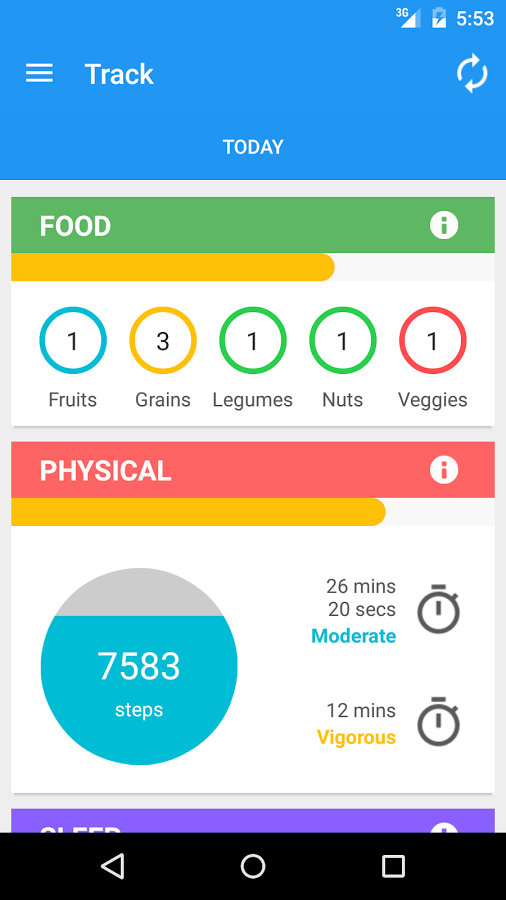
\includegraphics[width=\textwidth]{Files/prevention-study-3/figures/gm-new-log}
        \caption{Behavioural logging with real-time progress indicators}
        \label{fig: gm-new-log}
    \end{subfigure}
    \hfill
    \begin{subfigure}[t]{0.3\textwidth}
        \centering
        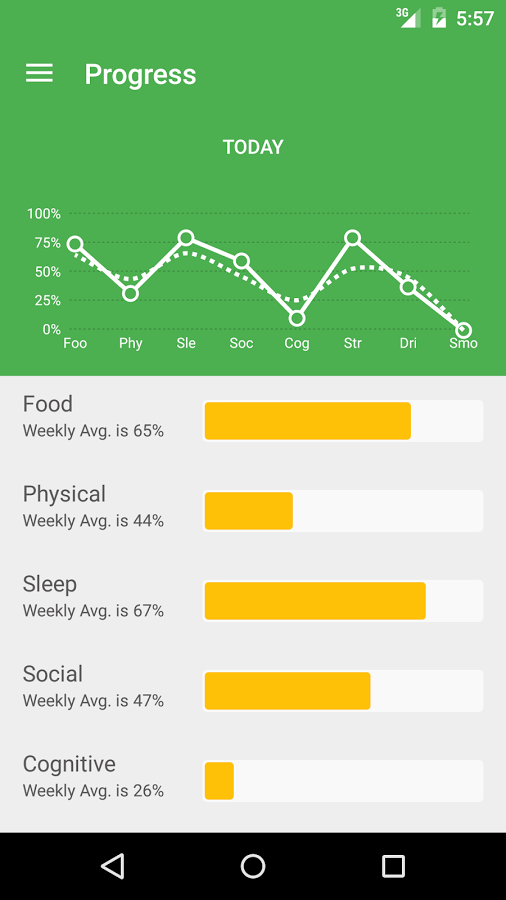
\includegraphics[width=\textwidth]{Files/prevention-study-3/figures/gm-new-performance}
        \caption{Showing current progress against their average performance}
        \label{fig: gm-new-performance}
    \end{subfigure}
    \caption{Screenshots of redesigned Gray Matters app, released to public as beta release on the android OS}
    \label{fig: graymatters-new}
\end{figure}

\begin{figure}[h]
    \centering
    \begin{subfigure}[t]{0.48\textwidth}
        \centering
        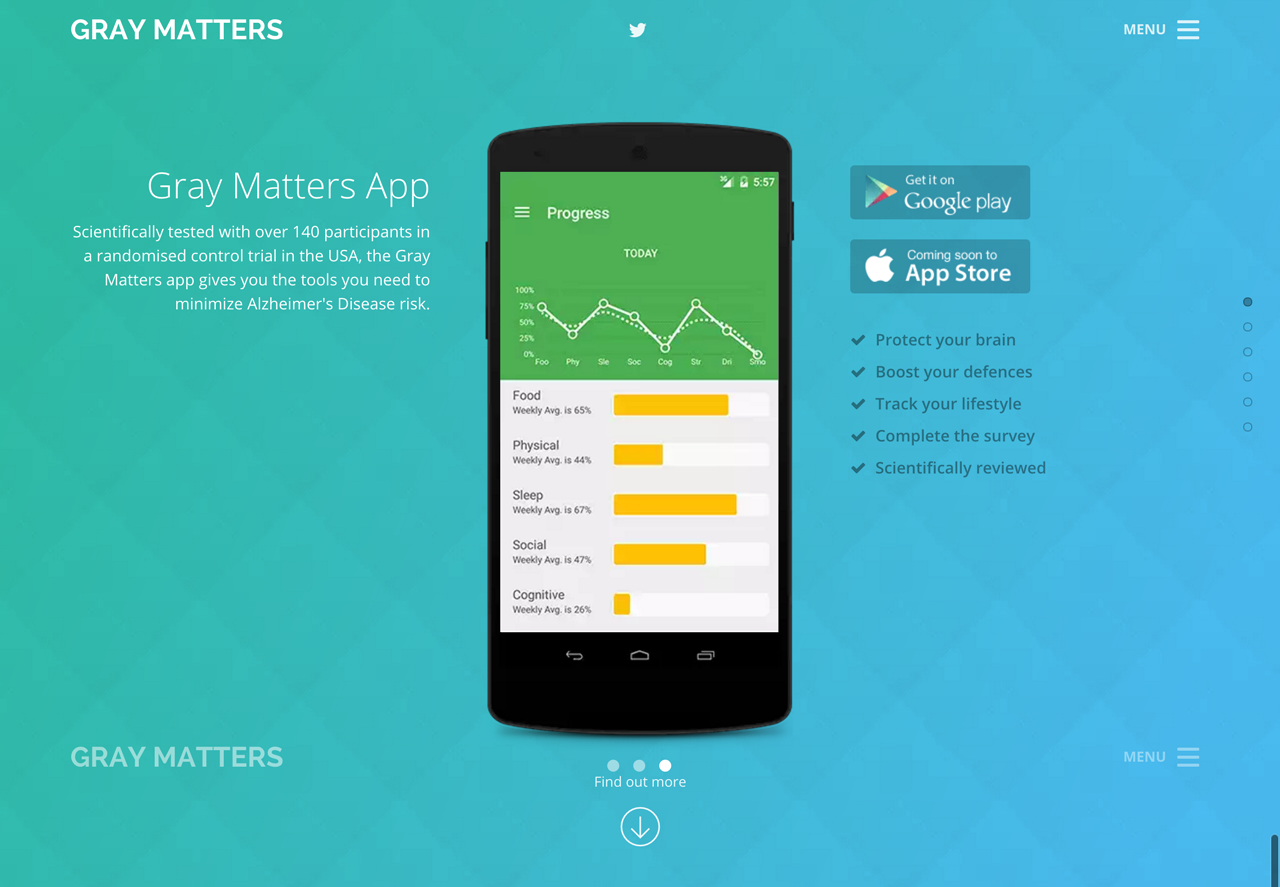
\includegraphics[width=\textwidth]{Files/prevention-study-3/figures/graymatters-web}
        \caption{graymattersapp.org screenshot}
        \label{fig: gm-web}
    \end{subfigure}
    \hfill
    \begin{subfigure}[t]{0.48\textwidth}
        \centering
        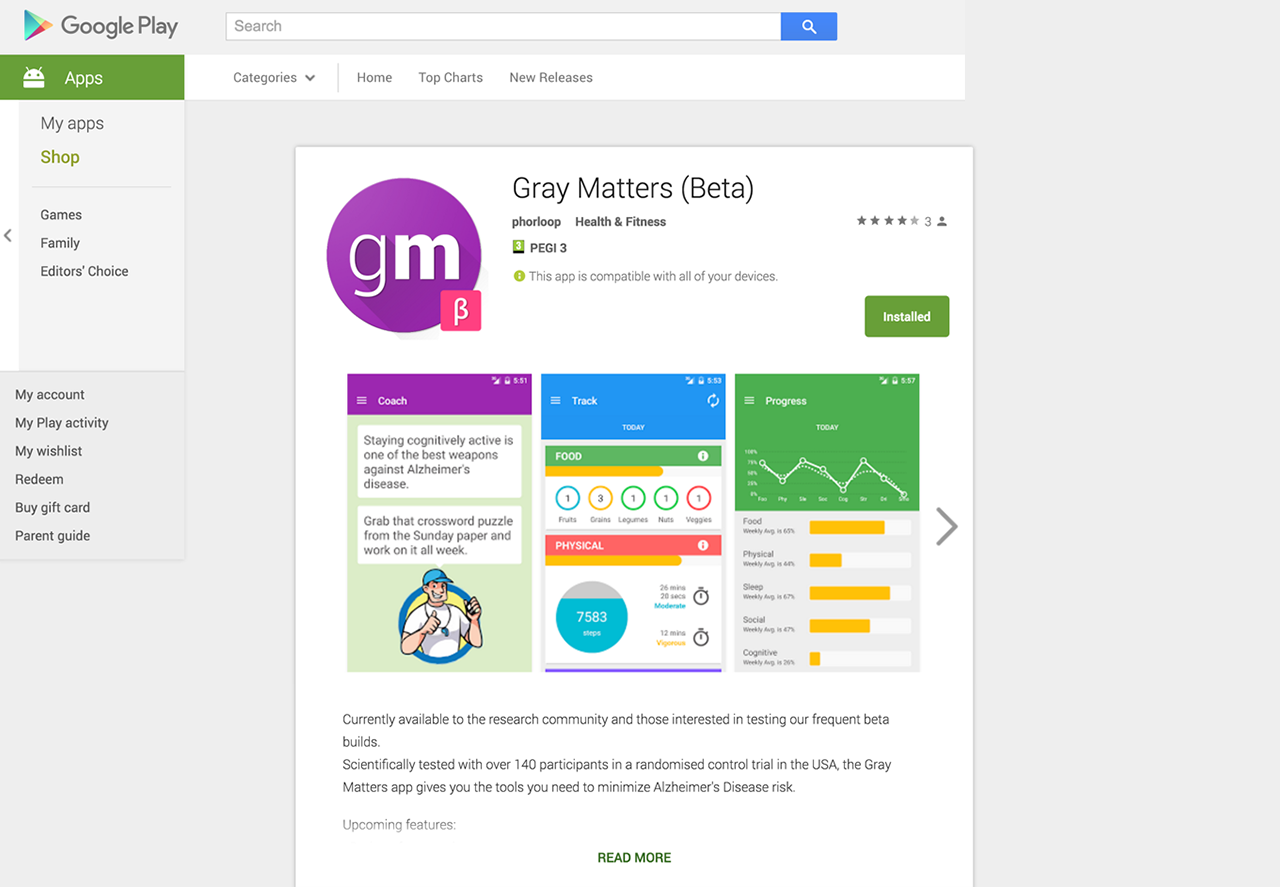
\includegraphics[width=\textwidth]{Files/prevention-study-3/figures/graymatters-playstore}
        \caption{Google Play app store}
        \label{fig: gm-playstore}
    \end{subfigure}
    \caption{Screenshots of dedicated Gray Matters app website and Google Play store listing}
    \label{fig: graymatters-online}
\end{figure}

The beta release was initially aimed to generate interest within the research and clinical domains, to encourage the creation of an intellectual consortium related to the works. However, many of those in the public domain were inspired by the media exposure and created a demand for access to the app as soon as possible, and subsequently it was made available as a free beta on the android play store.

\section{Closing Remarks}
This demand from the public emphasises the apparent need for a solution, especially from those who wish to take their overall health, including AD risk, into their own hands. It can be argued, as is often the case with new technology, that the most technologically capable will be those to benefit from it, and the rest of society will take years to adopt, or miss out completely. However, unlike technology platforms of the past, smartphones are now truly ubiquitous across all levels of society. With this in mind, and the increasing scientific literature supporting behaviour change and future disease risk increasing, it will not be long until it is the social norm for individuals to actively seek out personalised preventative medicine for specific diseases, and use an app to guide them on their quest for behaviour change.

With such a future envisaged, the previous 3 chapters have contributed to knowledge in the area by detailing a procedural framework to develop behaviour change apps, documented the development of an app by applying the framework, evaluated the resulting app with domain experts, and presented the clinical and behavioural results from a 6-month RCT using the app as an  intervention.
